%!TEX root = thesis.tex

\chapter{Spatial Awareness for Robot Cameras: Predicting images from topic context} \label{ch:spatial-prediction}

In this chapter we consider learning a feature function so that we can use our topic model to make spatial predictions in the raw data domain, as opposed to in the feature domain as we demonstrated in the last chapter. A motivating example is visual-semantic search with a robotic camera. Consider a camera that can actively look around its environment by controlling its pan and tilt angles as well as modifying the size of its field-of-view (FOV) by zooming. As it looks around it presents the user with the set of types of things it has seen (eg. sky, buildings, road, etc.). If we have an \emph{invertible} feature function, \emph{ie.} one where we can encode an image as a word distribution, but also decode a word distribution as the correct image, we can use a topic model to visualize the topics and present the user with this type of summary. Given images representing the types, the user may specify the mixture they would like to find with the robot camera. By using the spatial topic model, we find a spatially coherent topic map, and therefore predicting the topics without directly observing the image or making strong geometric assumptions is relatively straightforward. In this context, the robot camera can predict where the closest match to the desired image will be found and frame it directly rather than searching by physically moving the camera. Further, our algorithm can decode the predicted topics into a predicted feature distribution and in turn decode the predicted feature distribution into an image, revealing what it expects to see given the training data it has seen so far.

As we have discussed previously, the spatio-temporal topic model is a natural fit for unsupervised learning problems involving low-dimensional mixtures of high-level types. Further, because of the relative simplicity of the topic model, it can be trained online. Because a simple, interpretable latent space is a motivating factor, retraining the model for each new environment it encounters is desirable, and online learning is a key advantage of our method over more general but also more data intensive methods. As we will show, the combination of general learned features and an environment specific topic model lead to autoencoding performance gains compared to other techniques with similarly tiny latent spaces.

\section{Approach}
Two key pieces are needed for this application: a feature function that encodes the relevant visual-semantics paired with its inverse, to produce images from features, and a spatial model which can predict the topic distributions at unvisited poses.

\subsection{Learning an invertible word distribution function} \label{sec:learning-features}

Due to their relative ease of training, we consider using a convolutional autoencoder (CAE) model for this task. A CAE is a CNN that is trained to reproduce its inputs while also encoding them in a hidden representation, usually of much smaller size than the inputs. Typically CAEs feature a sequence of convolutions and downsampling operations, with a smallest hidden dimension of dimensionality in the hundreds. Although many variants exist, the simplest version, uses the loss $\mathcal{L}_{ae} = (x - d(e(x))^2$ where $e(x)$ is the encoding network and $d(z)$ the decoding network. After training, the representation $e(x)$ may be used as a feature vector for other tasks, or else included pre-trained as the first few layers of model for a supervised learning task that is difficult to train from scratch.

In order to learn a representation compatible with topic modelling, we develop a modified CAE, the Categorical Information Boost Autoencoder (CIB-AE), where the encoding can be seen as the parameter of a categorical or multinomial distribution so that it gives an image's word distribution directly. Similar to DNNs used for classification tasks, we simply apply the softmax function to the activations of a standard CNN architecture to produce such a distribution.

Through the Dirichet priors on topics and topic-word distributions, LDA descendants such as the spatio-temporal topic model make the implicit assumption that documents have sparse word distributions. Although we do not specify exactly how sparse such a sparse mixture of sparse multinomials is, we have found in practice that simply renormalizing the features of conventional autoencoders produces word-distributions that are too uniform to be modelled productively by LDA. Therefore, CIB-AE employs an additional loss term
\begin{equation}
    \mathcal{L}_{CIB} = \sum_{m=1}^M(x_m - d(e(x_m)))^2 - \lambda MI\left(x, w\right)
\end{equation}
where $w \sim e(x)$ and $MI$ stands for the mutual information, a measure of the degree if dependence between two random variables. Choosing a large value for $\lambda$, will result in representations that favor encoding distributions with high mutual information between images and encoding distributions, \emph{ie.} those where training images are as distinguishable as possible in encoding space. On the other hand, choosing a small $\lambda$ will result in encodings which may be very similar, but result in a low MSE. 

To illustrate how this loss works, consider that mutual information can be rewritten as $MI\left(x, w\right) = H[w] - H[w | x] $ where $H[w | x]$ signifies the conditional entropy of $w$ given $x$. By subtracting the mutual information from the loss, the $H[w | x]$ term ensures that individual encodings must have low-entropy, and are therefore sparse, while the $-H[w]$ term ensures that the overall distribution of encodings is high-entropy, and therefore as uniform as possible. The combination of these two terms means that the encodings must use different dimensions of the feature space, and ensure that image encodings are as distinct from one-another as possible.

Reorganizing the mutual information in this also way reveals how to estimate it from a minibatch of size $M$:
\begin{equation}
\begin{split}
    -MI\left(x, w\right) = H[w | x] - H[w] = \\
    \mathbb{E}_{w \sim e(x)}\left[ -\log p(w) \right] - \mathbb{E}_x\left[ \mathbb{E}_{w \sim e(x)}\left[ -\log p(w) \right] \right] \approx \\
    -\frac{1}{M} \sum_{m=1}^M \sum_{d=0}^V e(x_m)_d (\log e(x_m)_d) +
            \sum_{d=0}^V \overline{e(x)}_d \log \overline{e(x)}_d
    \end{split}
\end{equation}
where $\overline{e(x)}$ signifies the average encoding for the $M$ images in the batch. Clearly, estimating an expectation over the space of all possible training images with a minibatch of few dozen or at most a few hundred examples is crude. Nevertheless, the terms of this approximation naturally fit our goal of producing maximally sparse, maximally distinct encodings for as much of the training data as possible.

Our specific choice of architecutre is inspired by the feature layers of VGG \citep{Simonyan14c}. In particular, we choose a VGG-like encoder, followed by a dropout layer and a softmax function for the encoder, and a symmetric network of transposed convolutional layers for the decoder, following the approach of Segnet \citep{BadrinarayananK15} (See App.~\ref{ch:cibae-arch} for the full detail of our architecture). Our feature representation downsamples the image spatially by a factor of 32, while producing a 512 channel feature activation for each spatial region. All experiments are conducted with $128 \times 128 \times 3$ input images, resulting in $4 \times 4 \times 512 = 8192$ dimensional word distributions.

We find in practice that when the image space is normalized to the range $[-a,a]$, $\lambda = \frac{(2a)^2}{\log V}$ is a good choice, where $V$ is the dimension of the encodings \footnote{Note $\log V$ is the maximum possible entropy for a categorical distribution of dimension $V$, so this choice represents letting the MSE and MI terms have `equal' weight when both are in their worst cases}.

\subsection{Spatial topic prediction model}

Beyond simply finding any low-dimensional representation of the image space a robotic camera may encounter, the spatio-temporal topic model is able to learn such a representation that is also spatially coherent. We situate the topic model's neighborhoods in the space of poses, meaning that the resulting learned topic priors will form a map of the visually distinct regions in pan-tilt-zoom space.

Because our model is designed to make the topic priors locally smooth, we are able to develop a simple spatial prediction scheme for topic priors. Our spatial prediction model is fast to fit and run online, taking camera pose, learned topic prior pairs as training data, and predicting the topic prior for a test pose. We take inspiration from a nearest-neighbor model: in the simplest case our model is to predict the topic prior of the nearest training point for a test point. However, we envision using this system with only a few dozen training points, and would prefer predictions to degrade towards the global average topic distribution than a poor estimate of the topic prior when the test point is not near any training point.

To achieve this property, we make our predictions by a weighted sum over the topic distributions we have observed so far, where far training points have low weight and near training points have high weight. Rather than performing such a prediction with a direct mixture and renormalizing, we choose to implement the weighted sum in terms of the log-probability of each training topic, and then construct a predicted topic prior using the softmax function where the i-th dimension is defined as $\sigma(\theta)_i = \frac{\exp(\theta_i)}{\sum_{j=1}^{K} \exp(\theta_j)}$. We note that if the mixture of log-probabilities belongs to a valid probability distribution, the softmax function returns exactly that distribution. In addition, we define a weight function to produce the mixed log-probabilities as $\sigma\left(-D_X(x) \right)$ where $D_X(x)$ is some distance vector from a test point $x$ to all training points $X$. This choice of weight function has the appealing property that if one $D \approx 0$, all of the weight will be put on that training point. Further, with this weight function by controlling the scale of the distances we can control the sparsity of the weight vector; when the average distance is high the weights will be fairly uniform, while when the average distance is low, the weights will be sparser. Finally, we choose to use the plain $\mathit{L}_2^2$ distance between pan-tilt-zoom points as our distance function. However, in order to appropriately scale the distances and balance dimensions which may not truly incur equal loss of relevance for higher distances, we first scale the input points by the vector $w$ \footnote{Our distance could more precisely be called a Mahalanobis distance (normally formualted in terms of the covariance matrix $\Sigma = ww^T$)}. To summarize our prediction model:
\begin{equation}
\begin{split}
    D_X(x) = 
    \begin{bmatrix}
    \|w^Tx - w^T x_1 \|_2^2, & \|w^Tx - w^T x_2 \|_2^2, \ldots, \|w^Tx - w^T x_N \|_2^2
    \end{bmatrix}\\
    W(x) = \sigma \left( -D_{X}(x) \right)\\
    \theta(x) = \sigma \left( W(x) \log \left(\Theta_X \right) \right)
\end{split}
\end{equation}

Finally, we note that setting $w$ by hand is difficult as the best choice may vary from environment to environment, and is unnecessary, as both fitting and prediction are extremely efficient with this model. Instead, we choose to set $w$ by 2-fold cross validation. We exhaustively cover the 3d grid of values for each dimension of $w$, fitting and predicting for half the data for every parameter candidate. Then each parameter candidate is evaluated according to the mean Jenson-Shannon Divergence ($D_{JS}$) of its topic-prior predictions compared to the held-out topic-prior predictions. $D_{JS}$ is defined as:
\begin{equation}
D_{JS}\left[ p, q \right] = \frac{1}{2} \left(D_{KL}[p, m] + D_{KL}[q, m]\right)
\end{equation}
where $m = \frac{p+q}{2}$. While $D_{KL}[p,q]$ most directly measures the information lost by approxmating the true topic distribution with the prediction, $D_{JS}$ is a similar alternative, with the attractive properties of being symmetric, positive and bounded above that $D_{KL}$
 does not possess. 

\section{Experiments}

\subsection{Simulated Pan-Tilt-Zoom Camera Dataset}
\begin{figure}
    \centering
    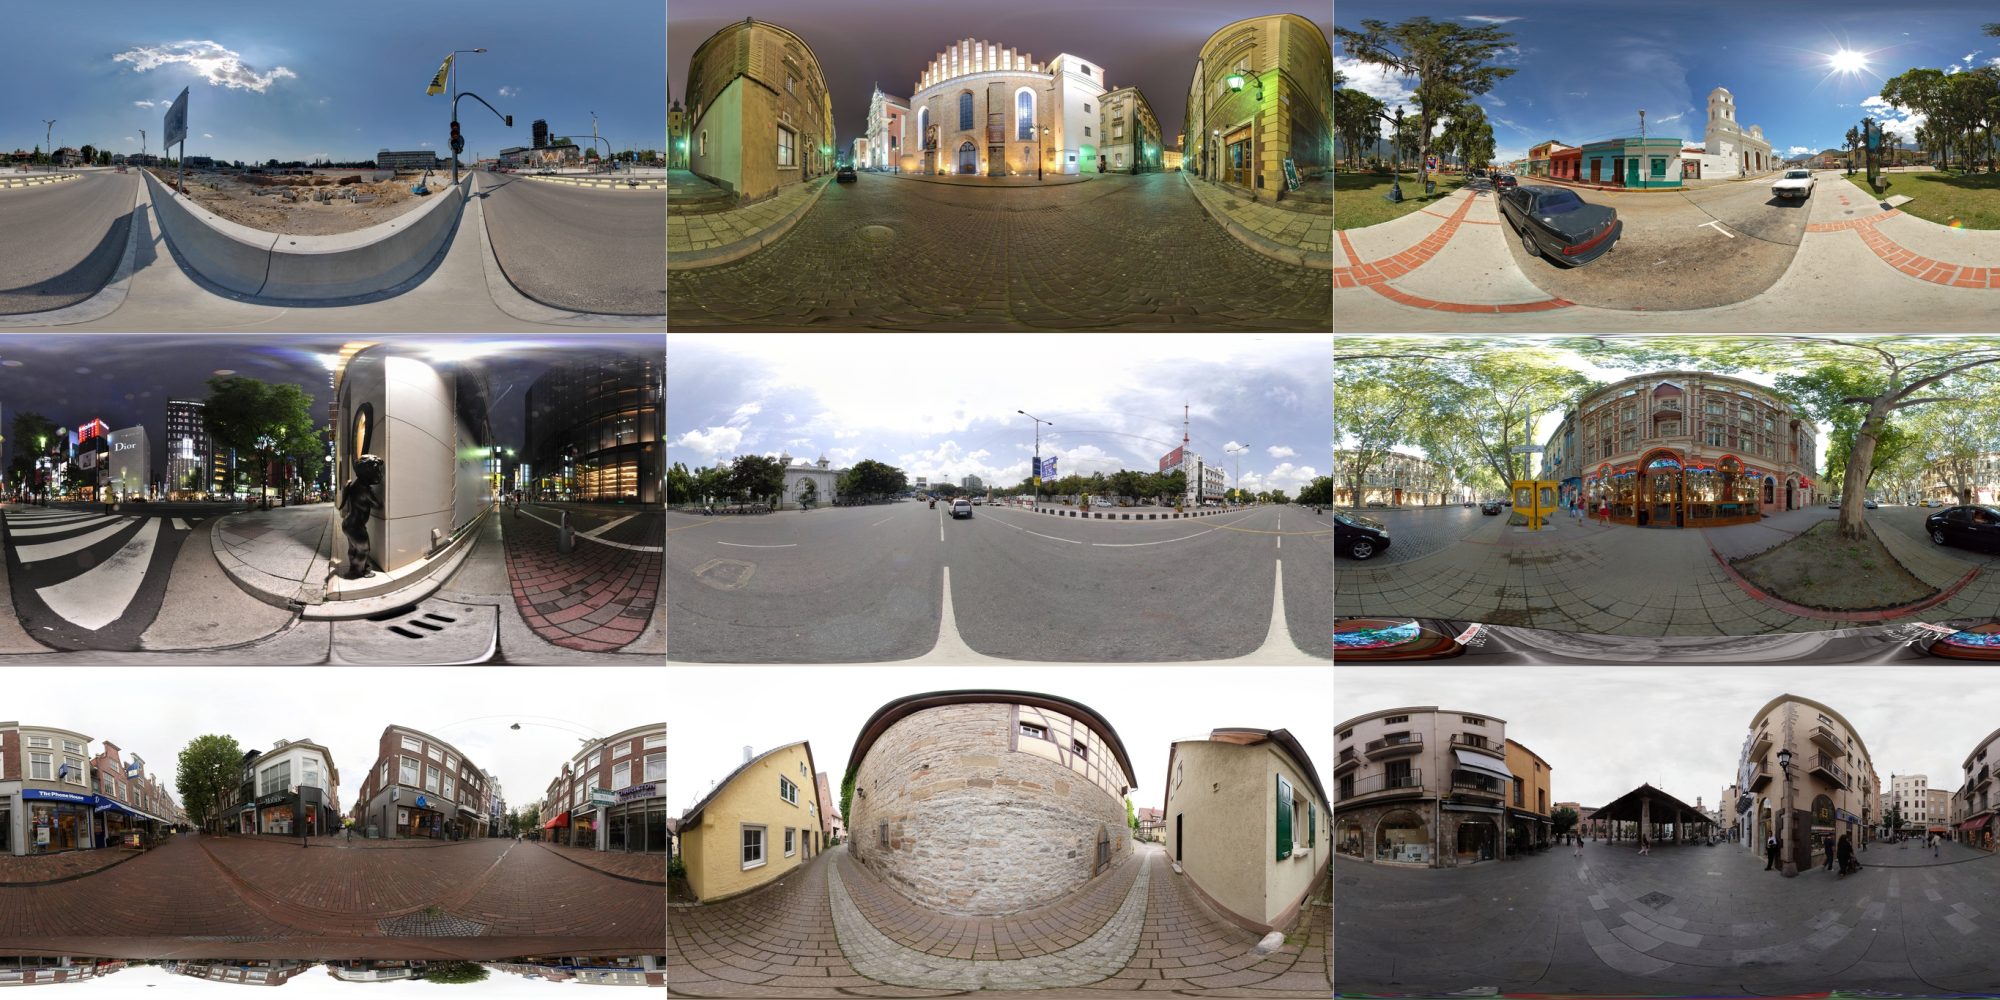
\includegraphics[width=0.85\textwidth]{figures/ptz/sun360_9x.png}
    \caption{Example 360 degree panoramas from the SUN360/street dataset.}
    \label{fig:sun360_ex}
\end{figure}

We demonstrate our approach with a simulated outdoor pan-tilt-zoom camera, using data from the `street' category of the SUN360 dataset \citep{SUN360}. Specifically SUN360/street comprises a dataset of 161 360 degree panoramas projected into rectangular $9104 \times 4552$ pixel images (Fig.~\ref{fig:sun360_ex}). These panoramas are taken in various cities and towns across the world, from street corners and from car-mounted cameras. We parameterize views in terms of tilt angle $T$, pan angle $P$, zoom factor $Z$. Given a base field-of-view (fov) $A_0$ and a target camera resolution, we compute the projection to the desired perspective $R = R_TR_P$ where
\begin{equation}
\begin{split}
R_T =& 
\begin{bmatrix}
1 & 0 & 0\\
0 & \cos(T) & -\sin(T)\\
0 & \sin(T) & \cos(T)
\end{bmatrix}\\
R_P =&  
\begin{bmatrix}
\cos(P)        & \sin(P) - \sin(T)            & \sin(P)\cos(T)\\
\sin(P)\sin(T) & \cos(P)\cos(T)^2(1 -\cos(P)) & \cos(T)\sin(T)(1-\cos(P))\\
\sin(P)\cos(T) & \sin(T)\cos(T)(1-\cos(P))    & \cos(P)+\sin(T)^2(1-\cos(P))
\end{bmatrix}
\end{split}
\end{equation}
Using the fov $A = A_0/Z$ and output image resolution, we represent the output pixel locations as pan-tilt rotations from the center $P$, $T$. Then, projection proceeds as rotation by $R$ and a lookup in the full panorama image for each pixel in the output image. In all our experiments we consider a base fov of 76 deg and zoom factors $Z \in (1, 12]$, similar to a standard commodity camera. Further, to avoid wrapping angles, we consider only $T \in [-60, 60]$ and $P \in [-120, 120]$ deg.

\subsection{Place-specific autoencoder}

A key advantage of the topic-model based approach is that it can be trained online, whereas this is not practical for large deep-networks. This means that rather than learning a single model which aims to produce a low-dimensional embedding of all possible images, our robotic camera system can learn a new, place specific model, and is thus required to represent a vastly simpler space of images.

Our approach delegates learning the globally-salient image embedding to the CIB-AE. In particular, we trained our feature model using epochs of 5000 random poses from 80 random SUN360/street panoramas. We found that choosing a new set of random training poses for each epoch was crucial, however we kept the validation set fixed throughout training. The perspective projection described in the previous section is time consuming for high-resolution images, especially for those that do not fit in GPU memory. Therefore we trained for 175 epochs on random rectangular crops from the warped panorama images, and then 25 more epochs on projections to fine-tune the results. We achieved our results using the adaptive learning rate optimizer Adam~\citep{KingmaAdam}, however found that a learning rate decay by a factor of 0.9 every 10 epochs was also necessary. Example input images and their autoencoded counterparts can be seen in Fig.~\ref{fig:cibae_encodings}. We found the mean entropy of image encodings from 1000 random poses from the test set to be 2.335, or approximately equivalent to a uniform PMF over just 11 dimensions. On the other hand, the entropy of the mean encoding distribution from these 1000 examples was 8.769, whereas the maximum possible entropy where all feature dimensions were used uniformly would have had an entropy of 9.011.

\begin{figure}
    \centering
    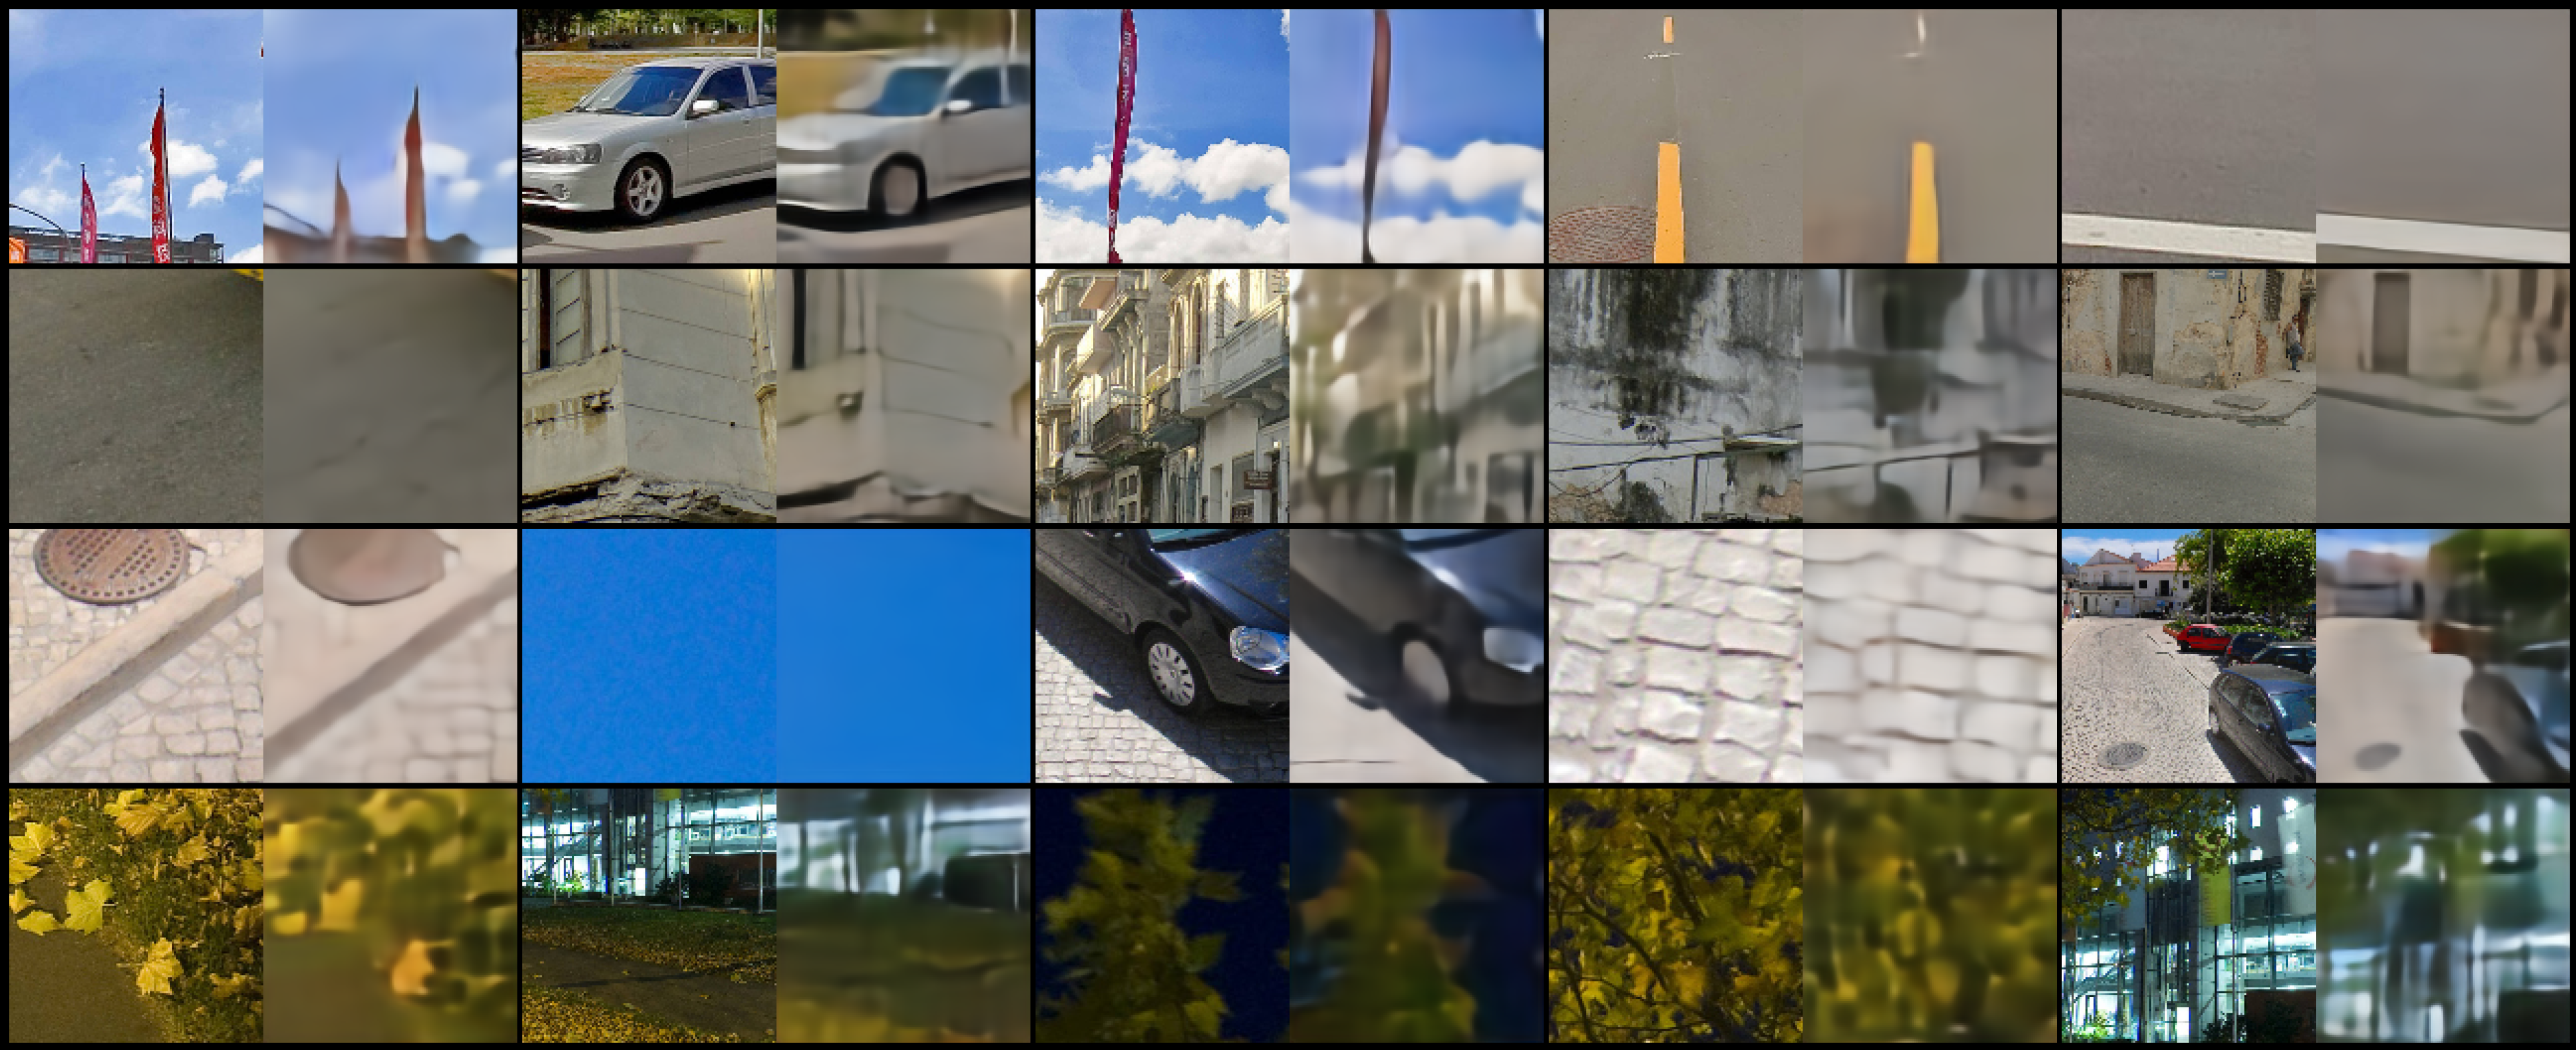
\includegraphics[width=\textwidth]{figures/ptz/mc3ae_encodings}
    \caption{Random example input images (left) and CIB-AE reconstructions (right) for 4 worlds (rows) from the SUN360/street test set.}
    \label{fig:cibae_encodings}
\end{figure}

Given the trained CIB-AE and a test environment, we train a spatio-temporal topic model with $K = 25$ topics, and neighborhoods of size 10 deg $\times$ 20 deg $\times$ 6 (tilt $\times$ pan $\times$ zoom). This neighborhood size choice corresponds to the intuition that environments are semantically `smoother' in tilt than pan, and much smoother while zooming than moving the camera. We chose concentration parameter values $\alpha = 0.2, \beta = 0.2$. We performed extensive cross validation on these parameter values and certain other choices were found to be good for particular environments, however we found that on average over a validation set of 20 environments these parameters gave the best performance.

We train the topic model at 0.5 hz, alternating randomly selecting a view, projecting its image and extracting its encoding distribution with refining the topic model. At the end of each refinement phase we fit the topic map described above to all of the previously observed pose, topic prior pairs. Similar to Ch.~\ref{ch:plankton}, we predict the encoding distribution for a new view x by first predicting the topic prior $ \hat{\theta} = \theta (x)$, and then taking the product with the MAP topic distribution matrix $ \hat{\theta} \Phi$.

\citep{vqvae2017}

\begin{figure}
    \begin{minipage}{0.55\textwidth}
        \subfloat[][]{
            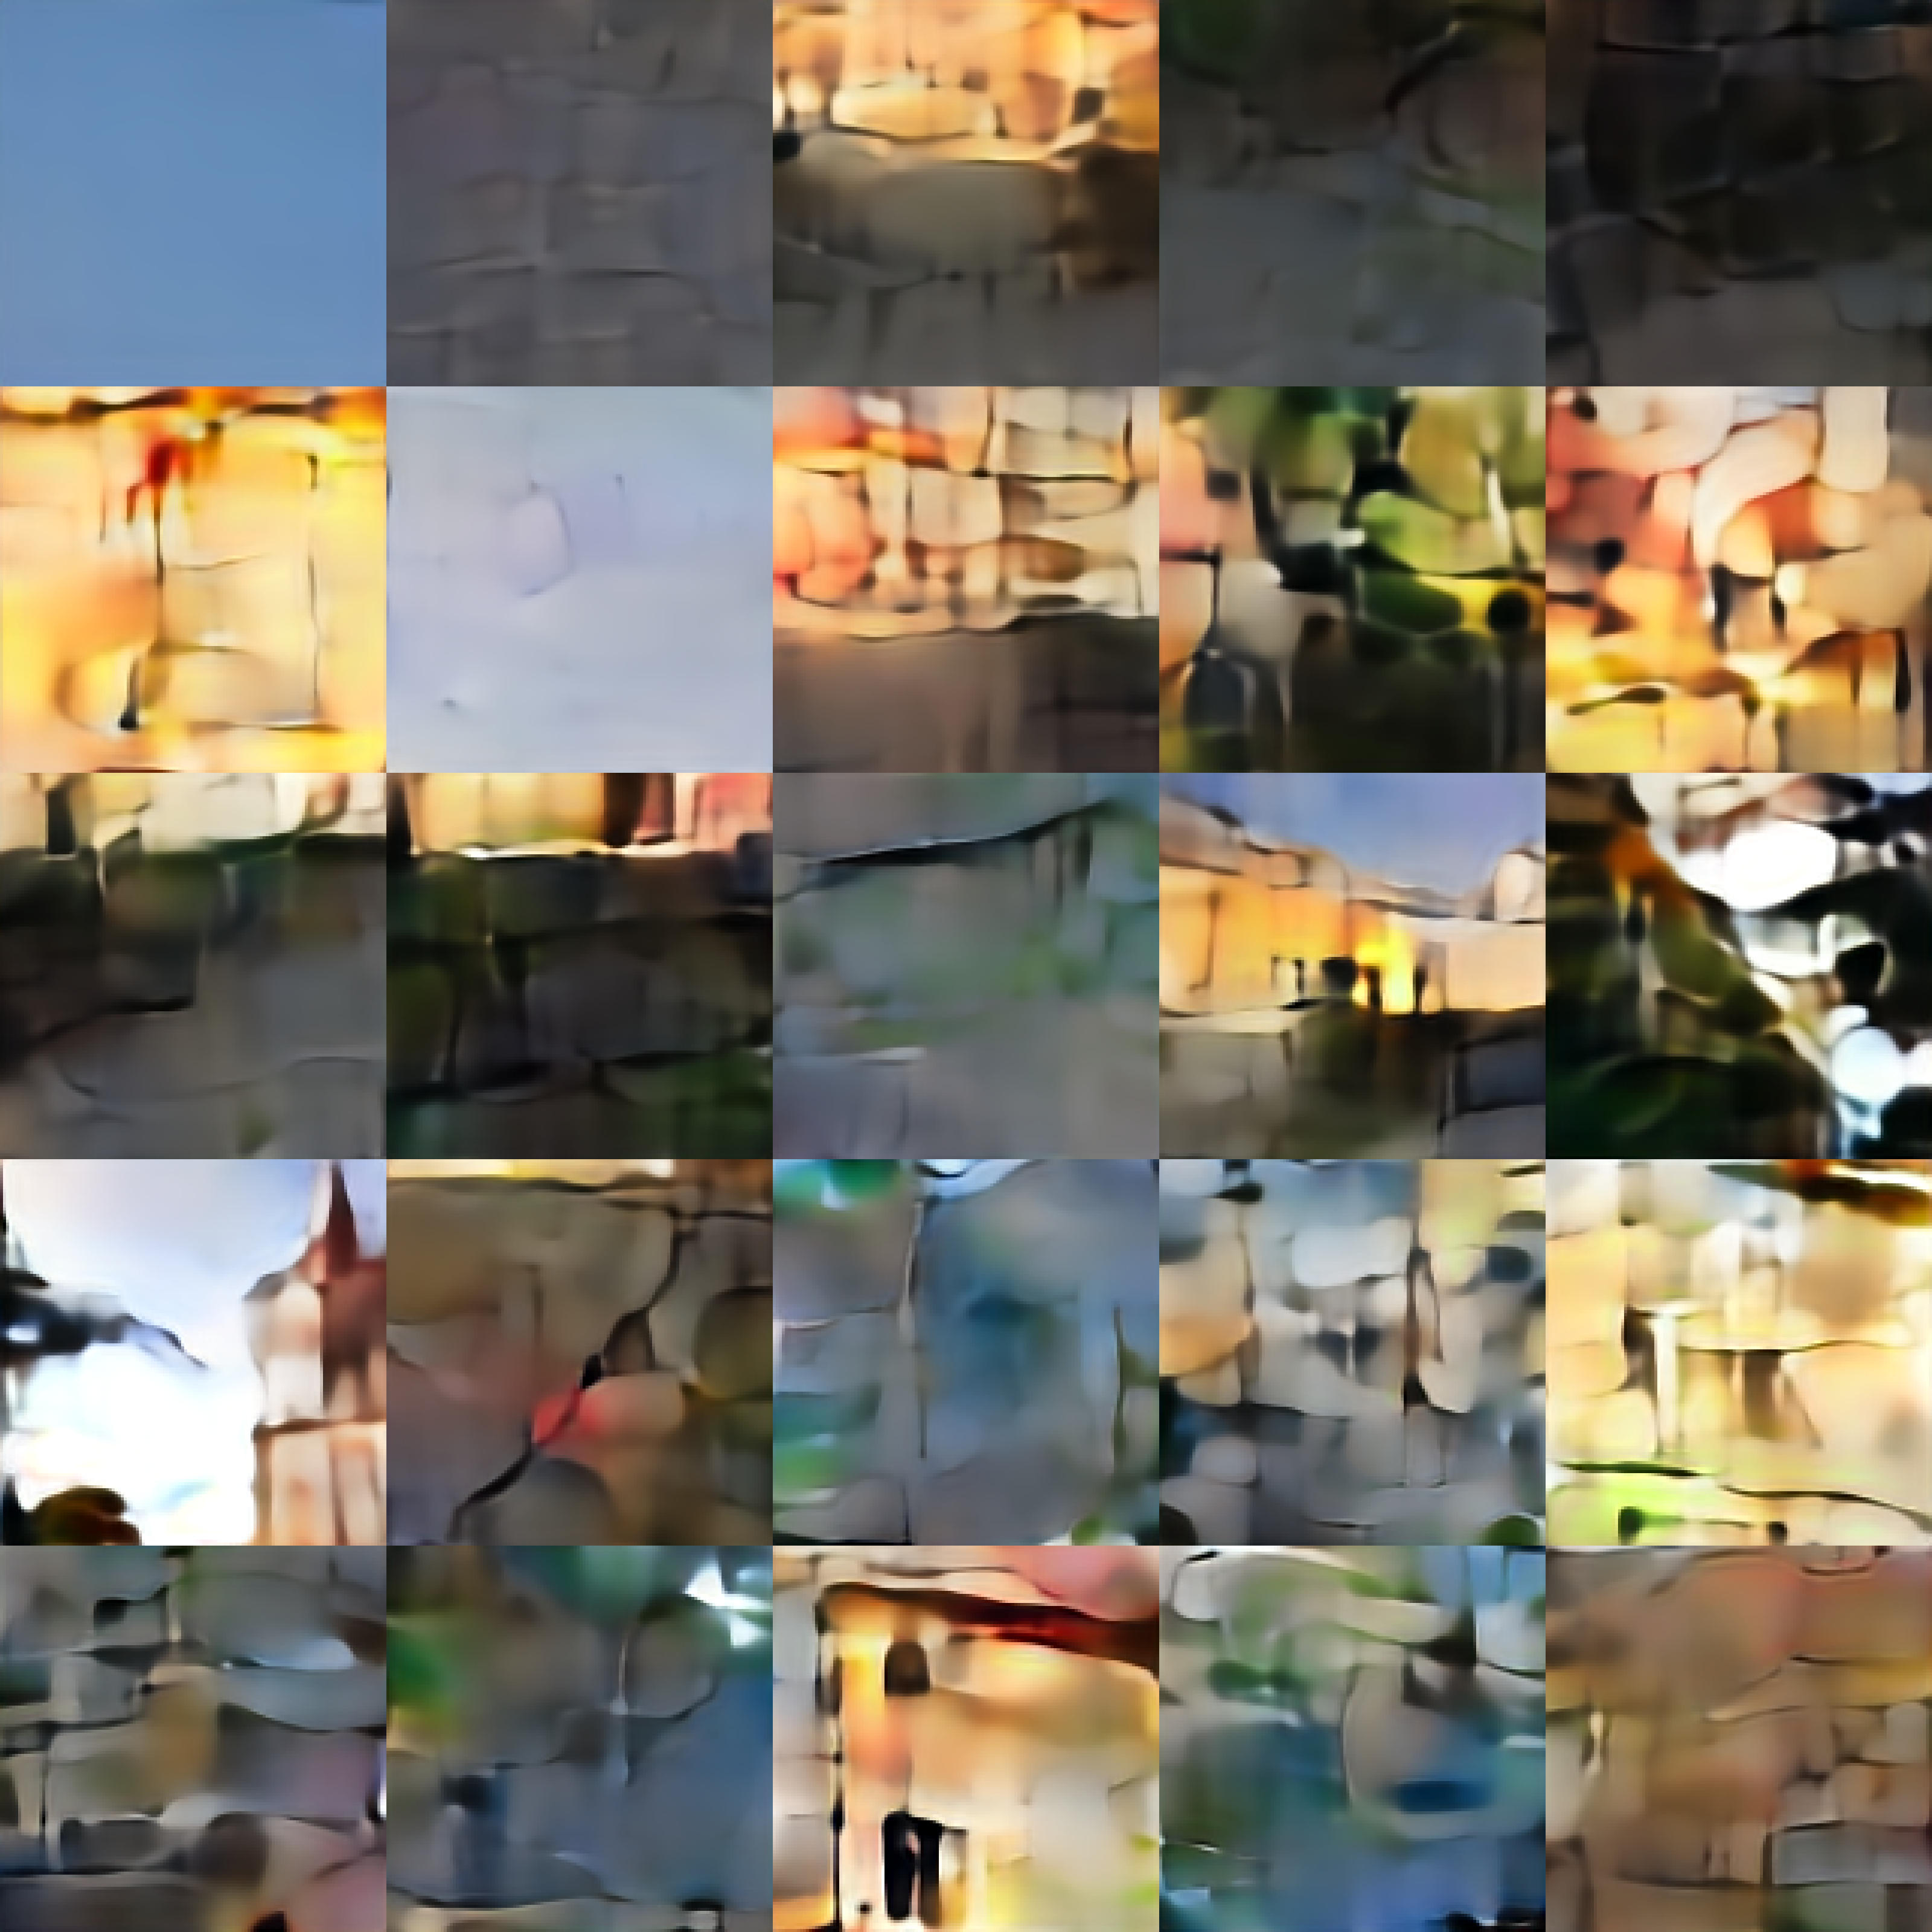
\includegraphics[width=\columnwidth]{figures/ptz/pano_7_topics.png}
            \label{fig:pano-7-topics}
        }
    \end{minipage} \hfill
    \begin{minipage}{0.44\textwidth}
        \subfloat[][]{
            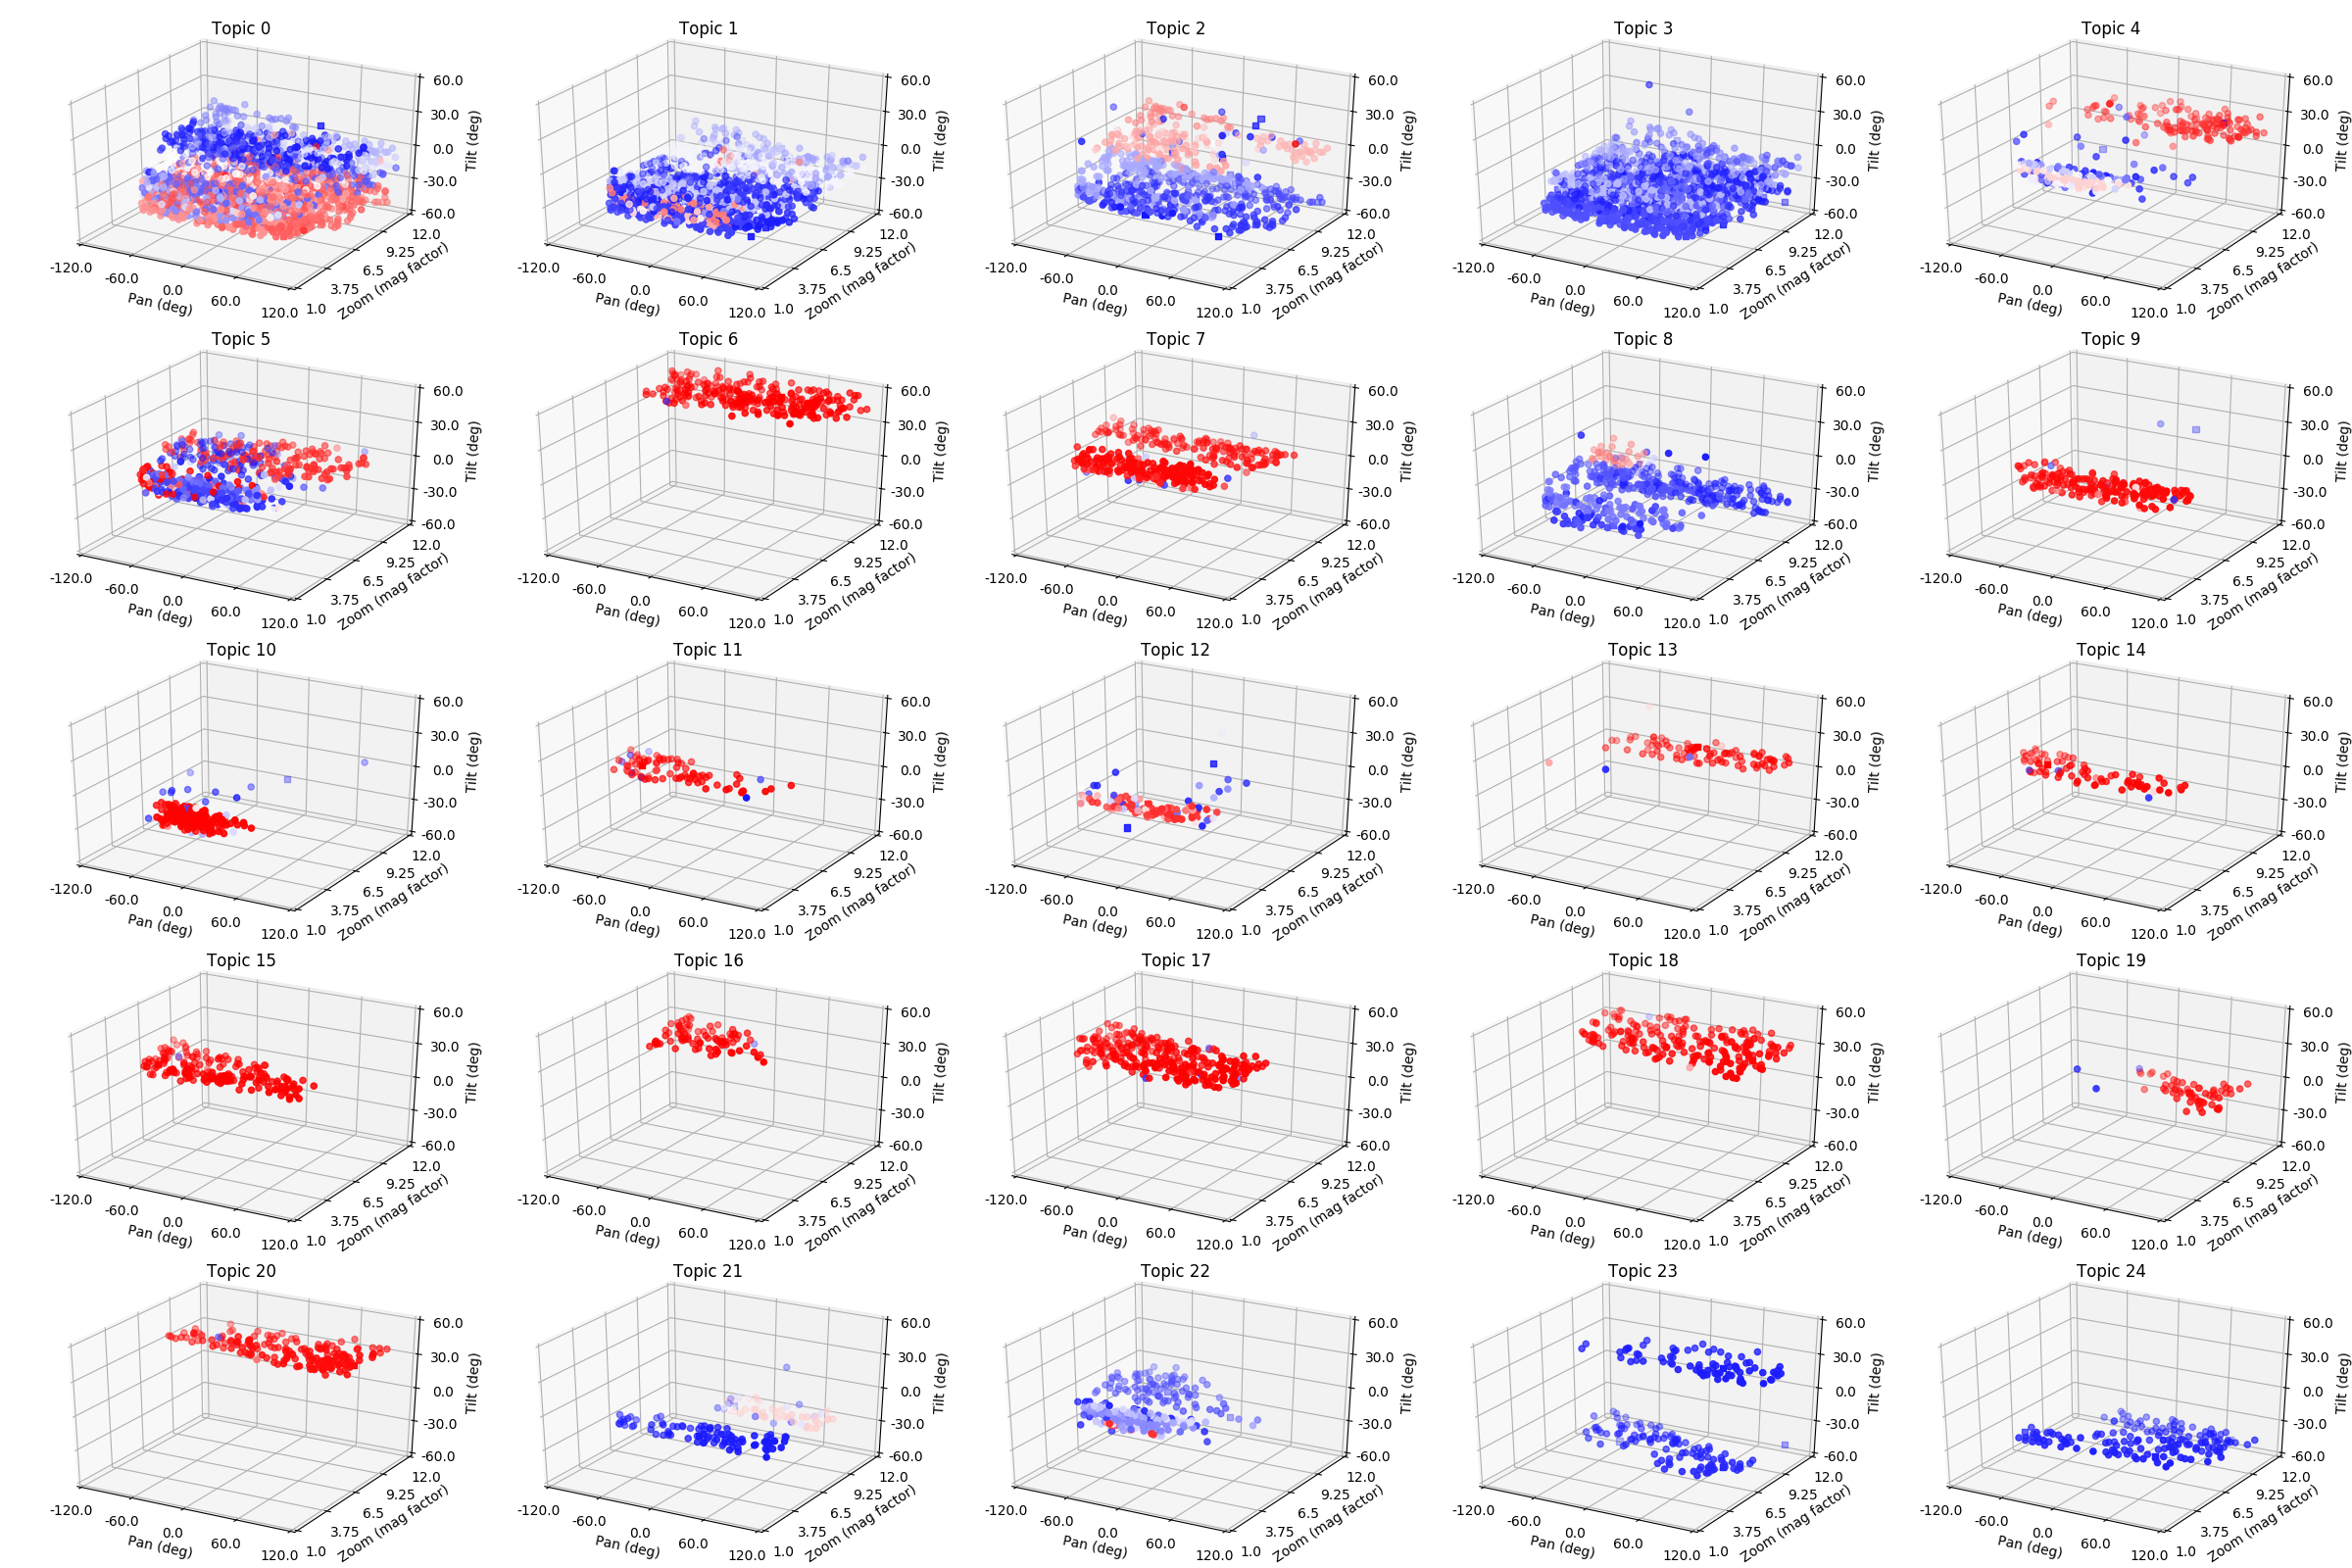
\includegraphics[width=\columnwidth]{figures/ptz/pano_7_map.png}
            \label{fig:pano-7-map}
        } \\
        \subfloat[][]{
            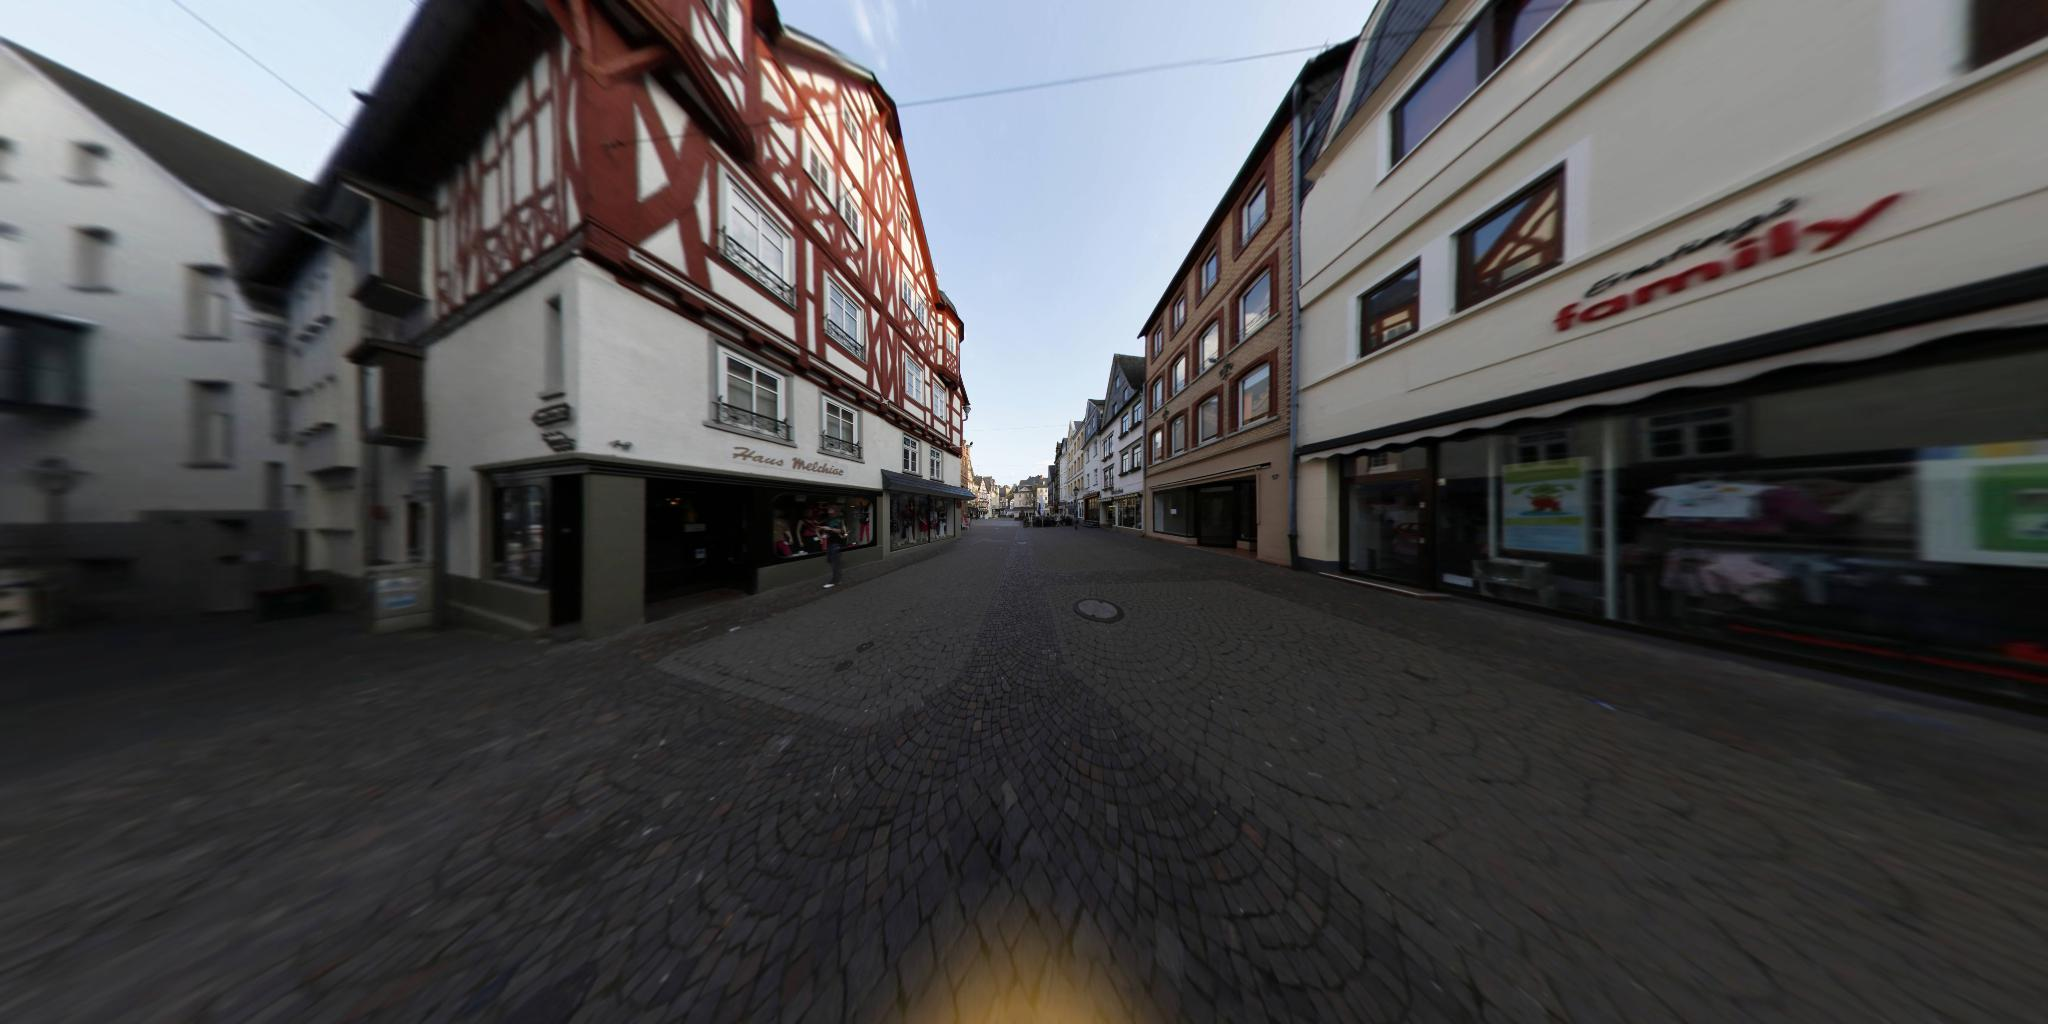
\includegraphics[width=\columnwidth]{figures/ptz/pano_7_pano.jpg}
            \label{fig:pano-7-pano}
        }
    \end{minipage}
    
    \caption{Example spatial prediction model after 50 training observations. \protect\subref{fig:pano-7-pano}} Fish-eye view of the entire panorama \protect\subref{fig:pano-7-topics}, Direct decoding of each topic-distribution ($\Phi_k$), And \protect\subref{fig:pano-7-map} predicted mixture of each topic.
    \label{fig:pano-7}
\end{figure}

\begin{figure}
    \begin{minipage}{0.55\textwidth}
        \subfloat[][]{
            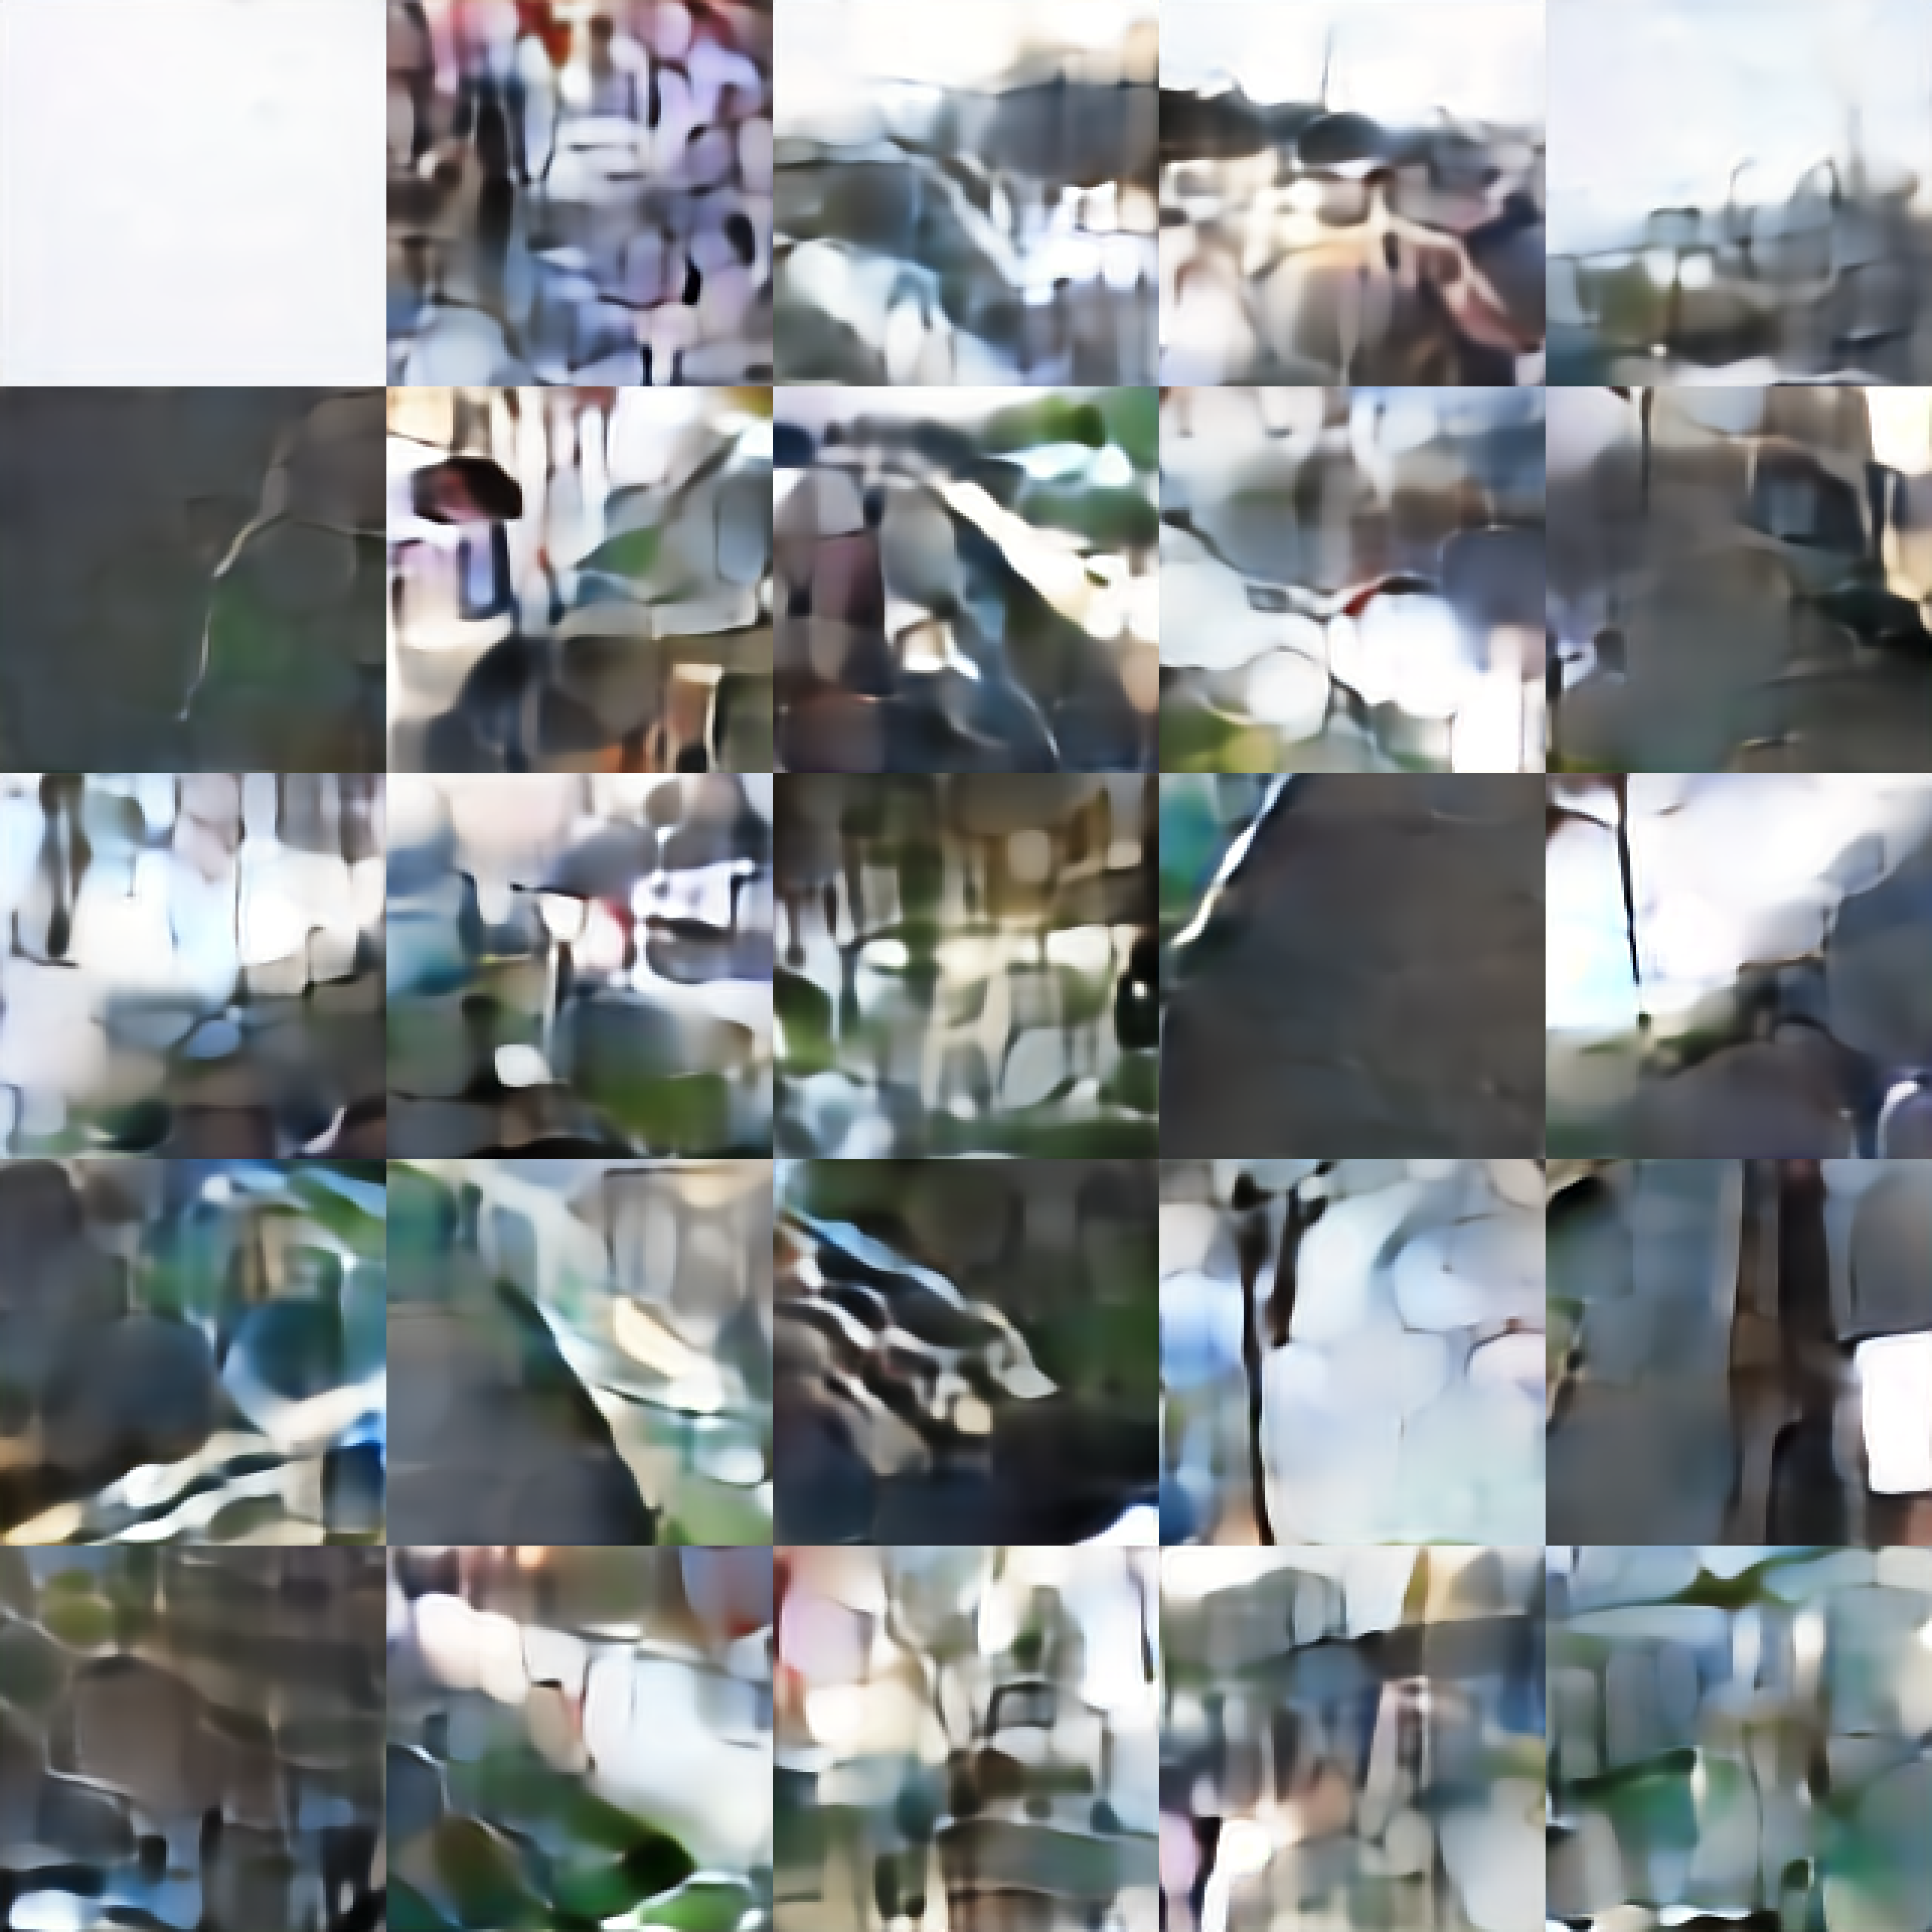
\includegraphics[width=\columnwidth]{figures/ptz/pano_15_topics.png}
            \label{fig:pano-15-topics}
        }
    \end{minipage} \hfill
    \begin{minipage}{0.44\textwidth}
        \subfloat[][]{
            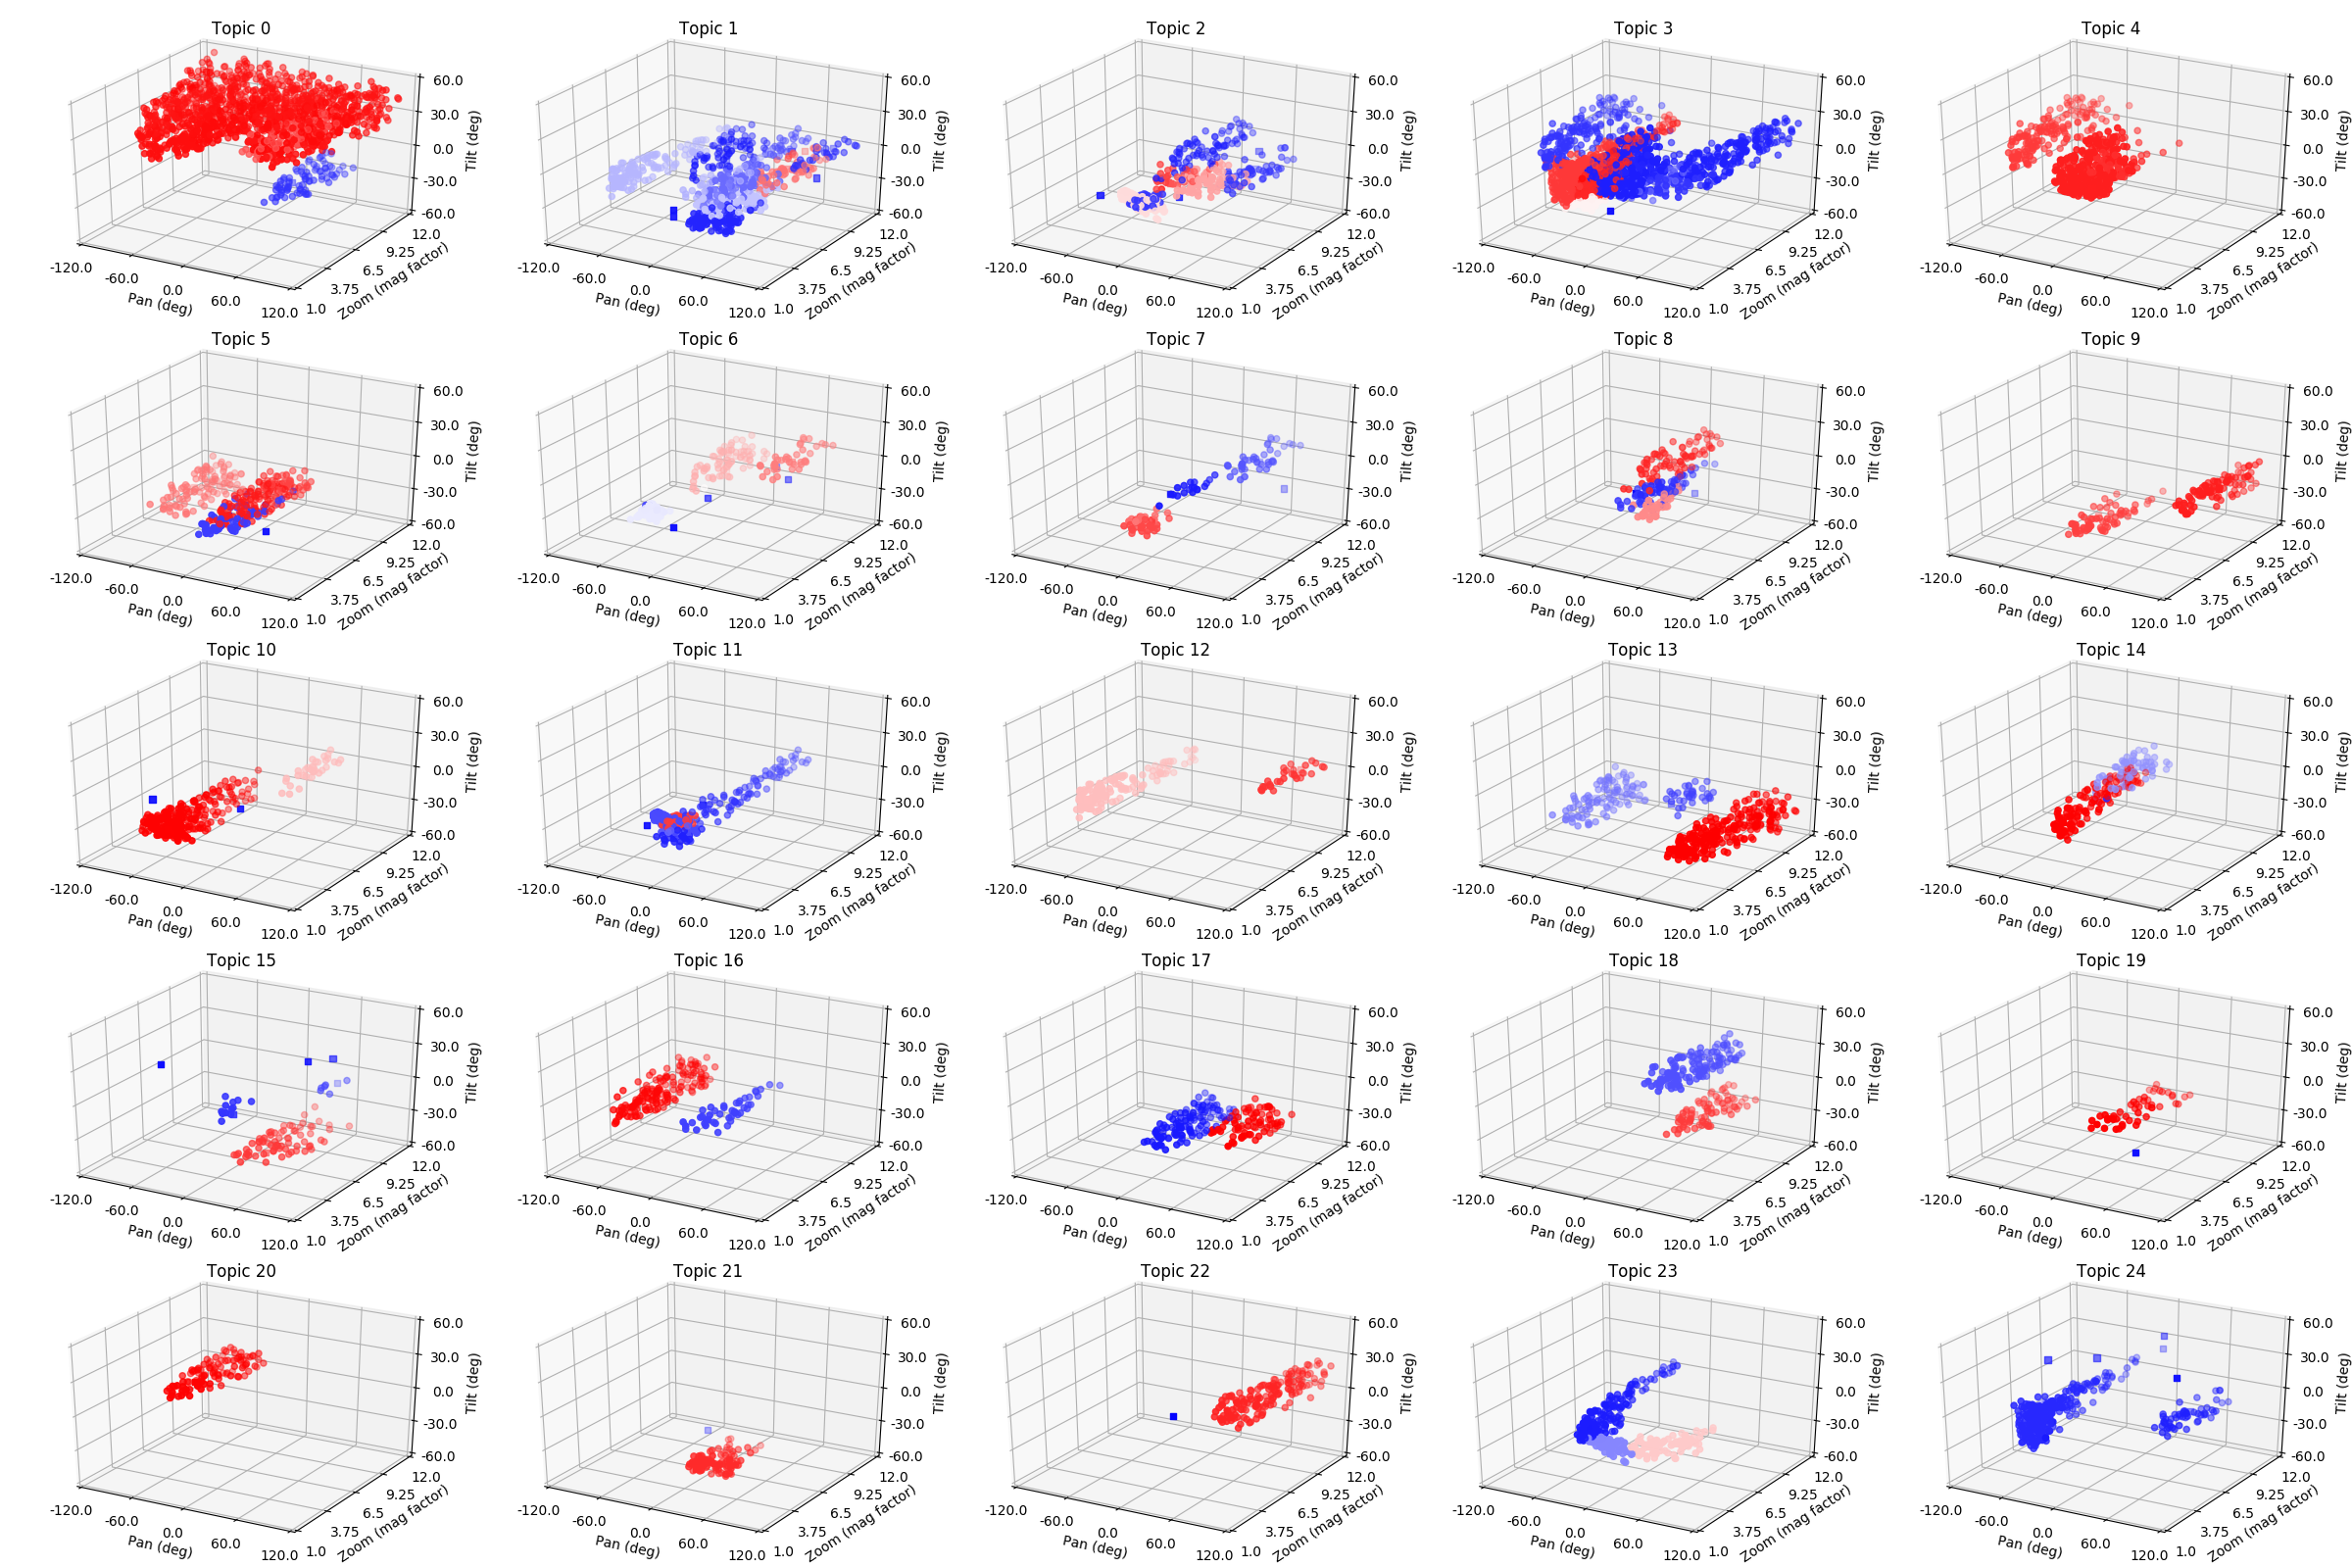
\includegraphics[width=\columnwidth]{figures/ptz/pano_15_map.png}
            \label{fig:pano-15-map}
        } \\
        \subfloat[][]{
            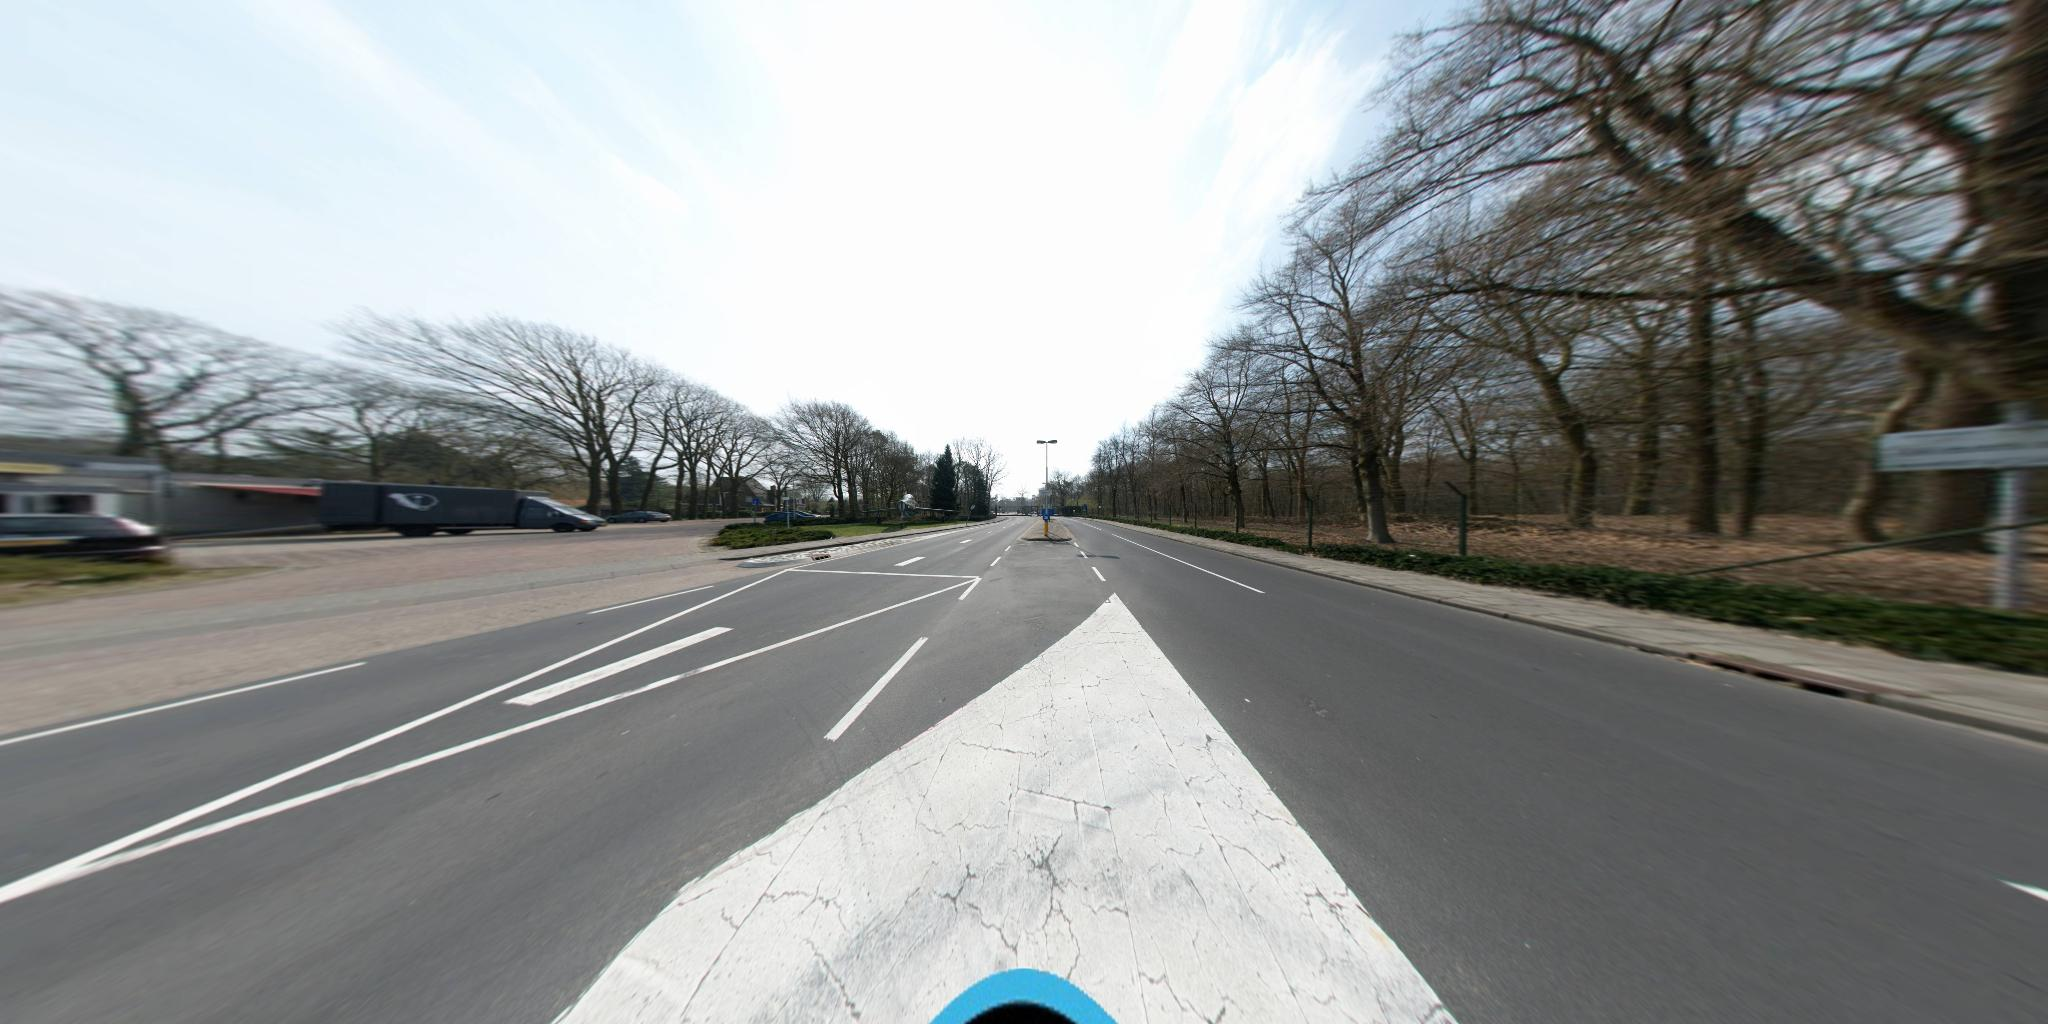
\includegraphics[width=\columnwidth]{figures/ptz/pano_15_pano.jpg}
            \label{fig:pano-15-pano}
        }
    \end{minipage}
    
    \caption{Example spatial prediction model after 50 training observations. \protect\subref{fig:pano-15-pano}} Fish-eye view of the entire panorama \protect\subref{fig:pano-15-topics}, Direct decoding of each topic-distribution ($\Phi_k$), And \protect\subref{fig:pano-15-map} predicted mixture of each topic.
    \label{fig:pano-15}
\end{figure}

\begin{figure}
    \begin{minipage}{0.55\textwidth}
        \subfloat[][]{
            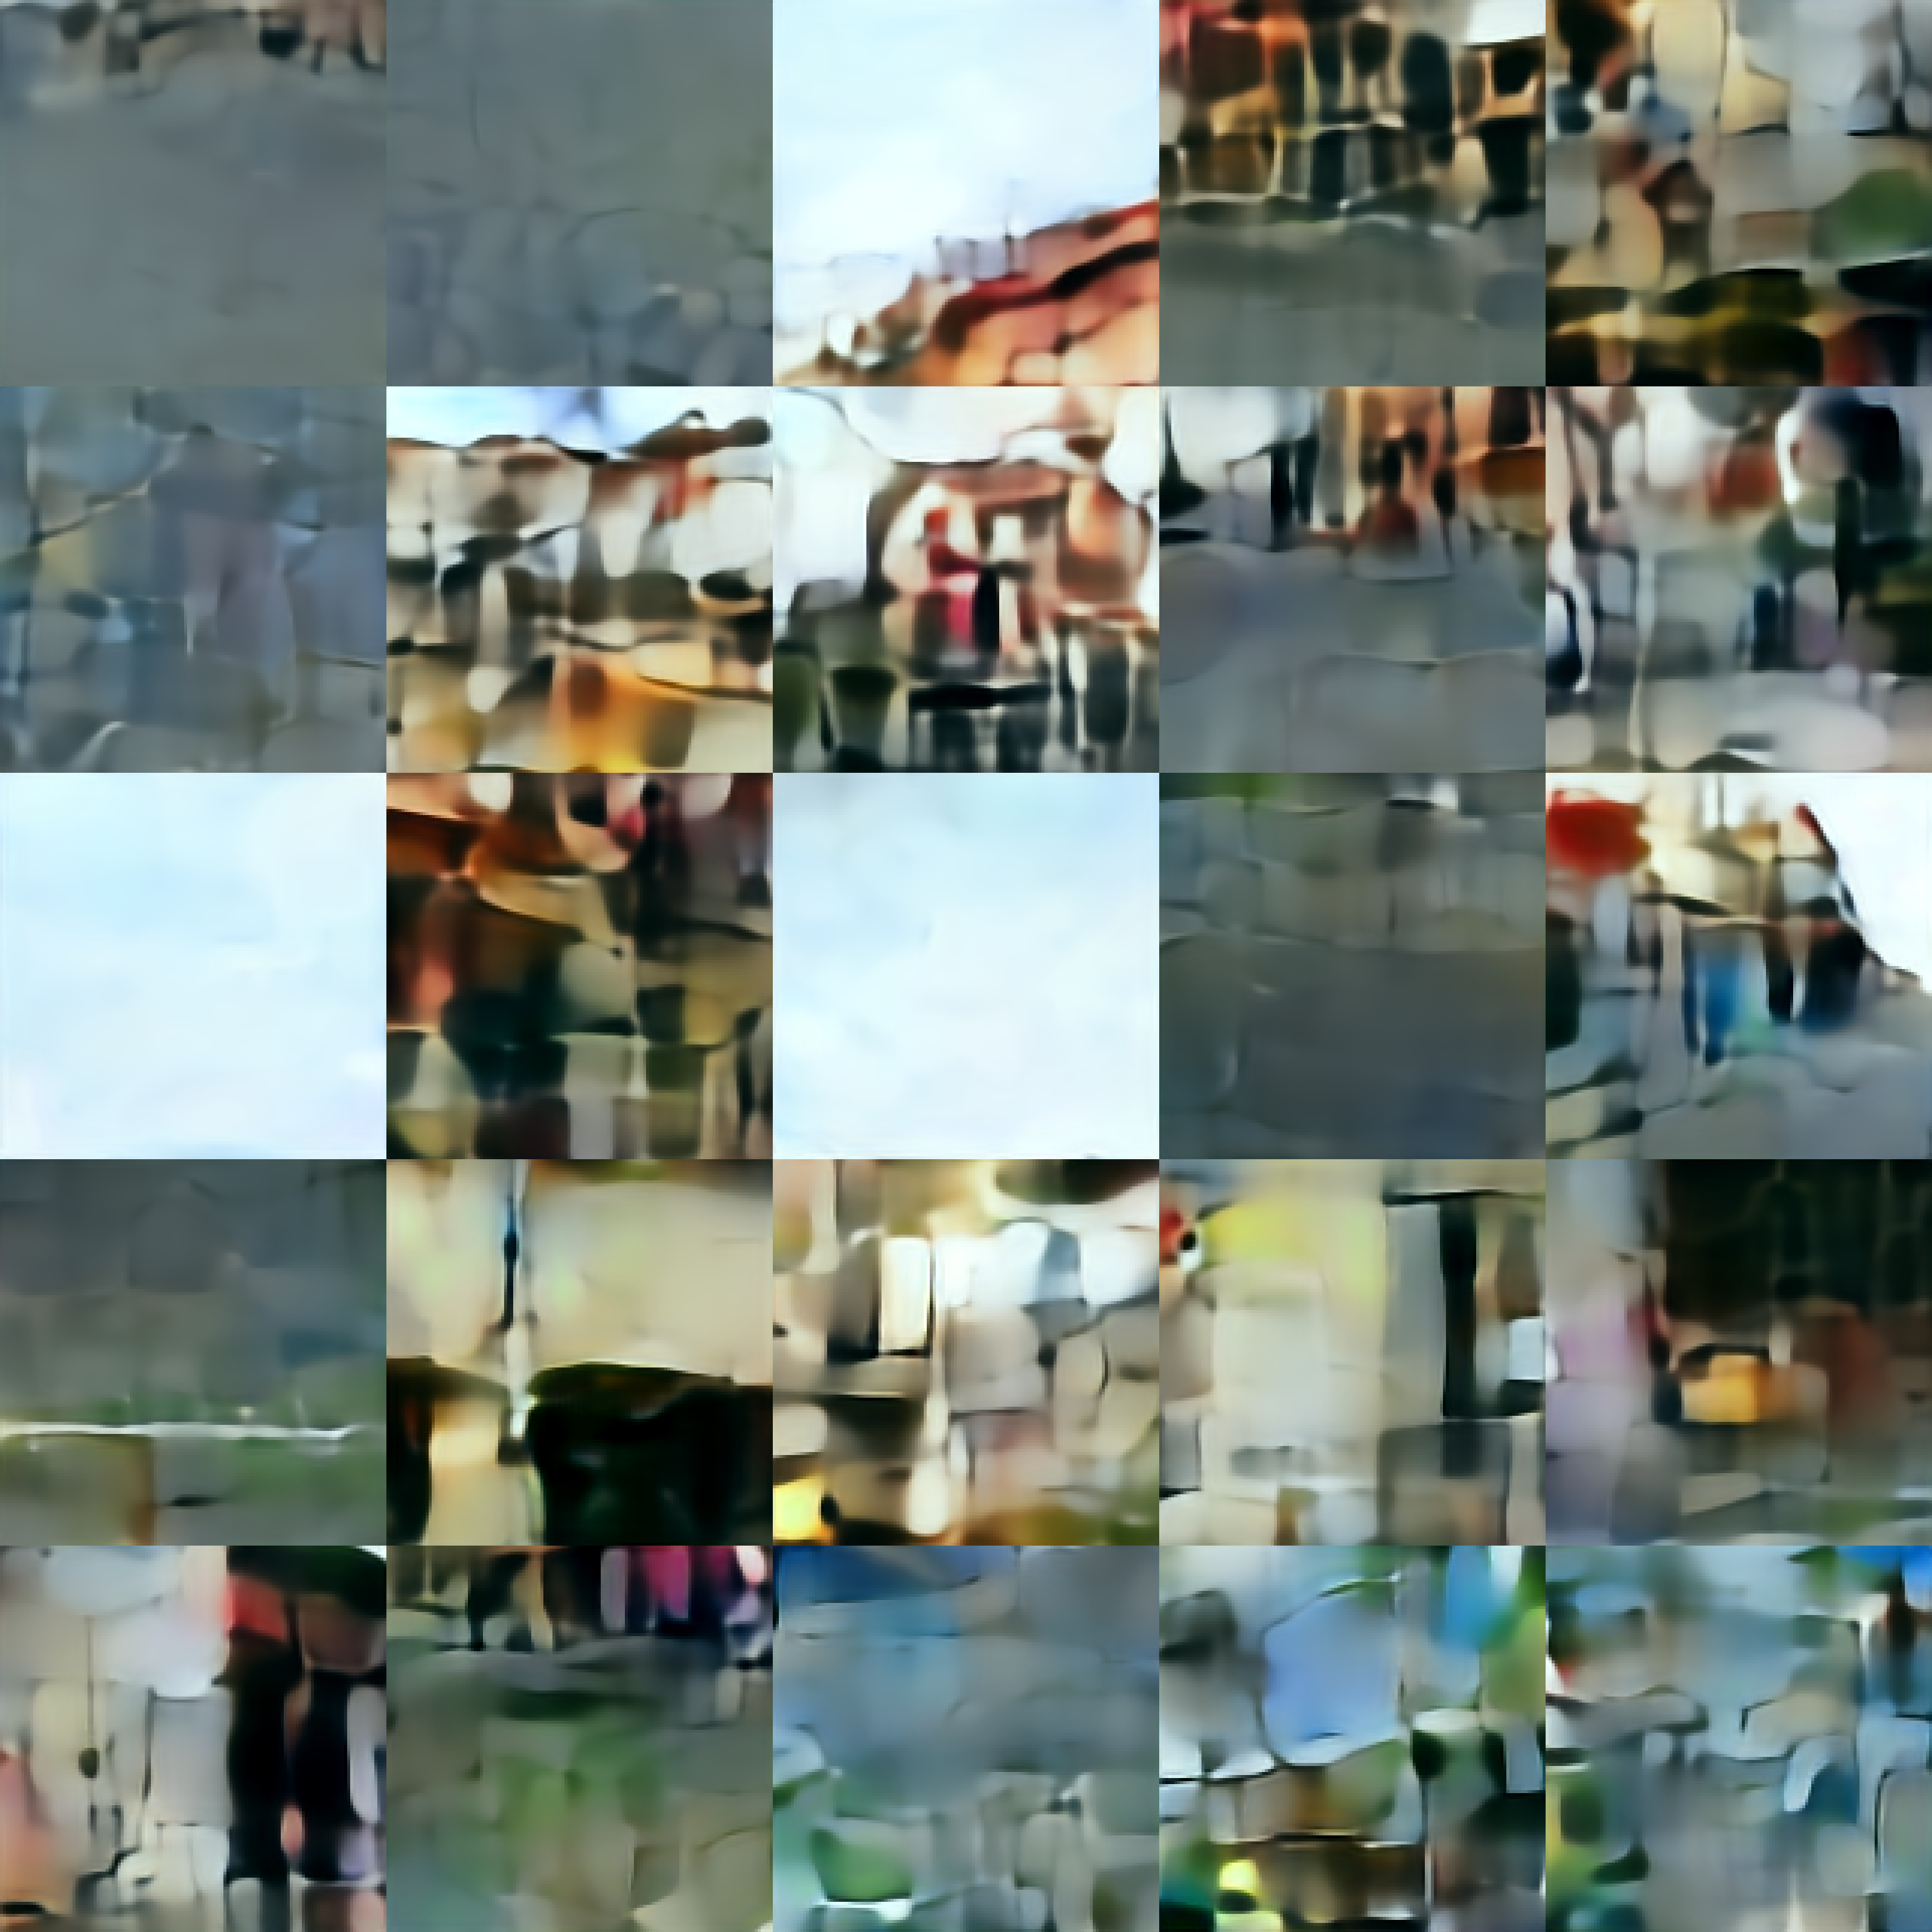
\includegraphics[width=\columnwidth]{figures/ptz/pano_24_topics.png}
            \label{fig:pano-24-topics}
        }
    \end{minipage} \hfill
    \begin{minipage}{0.44\textwidth}
        \subfloat[][]{
            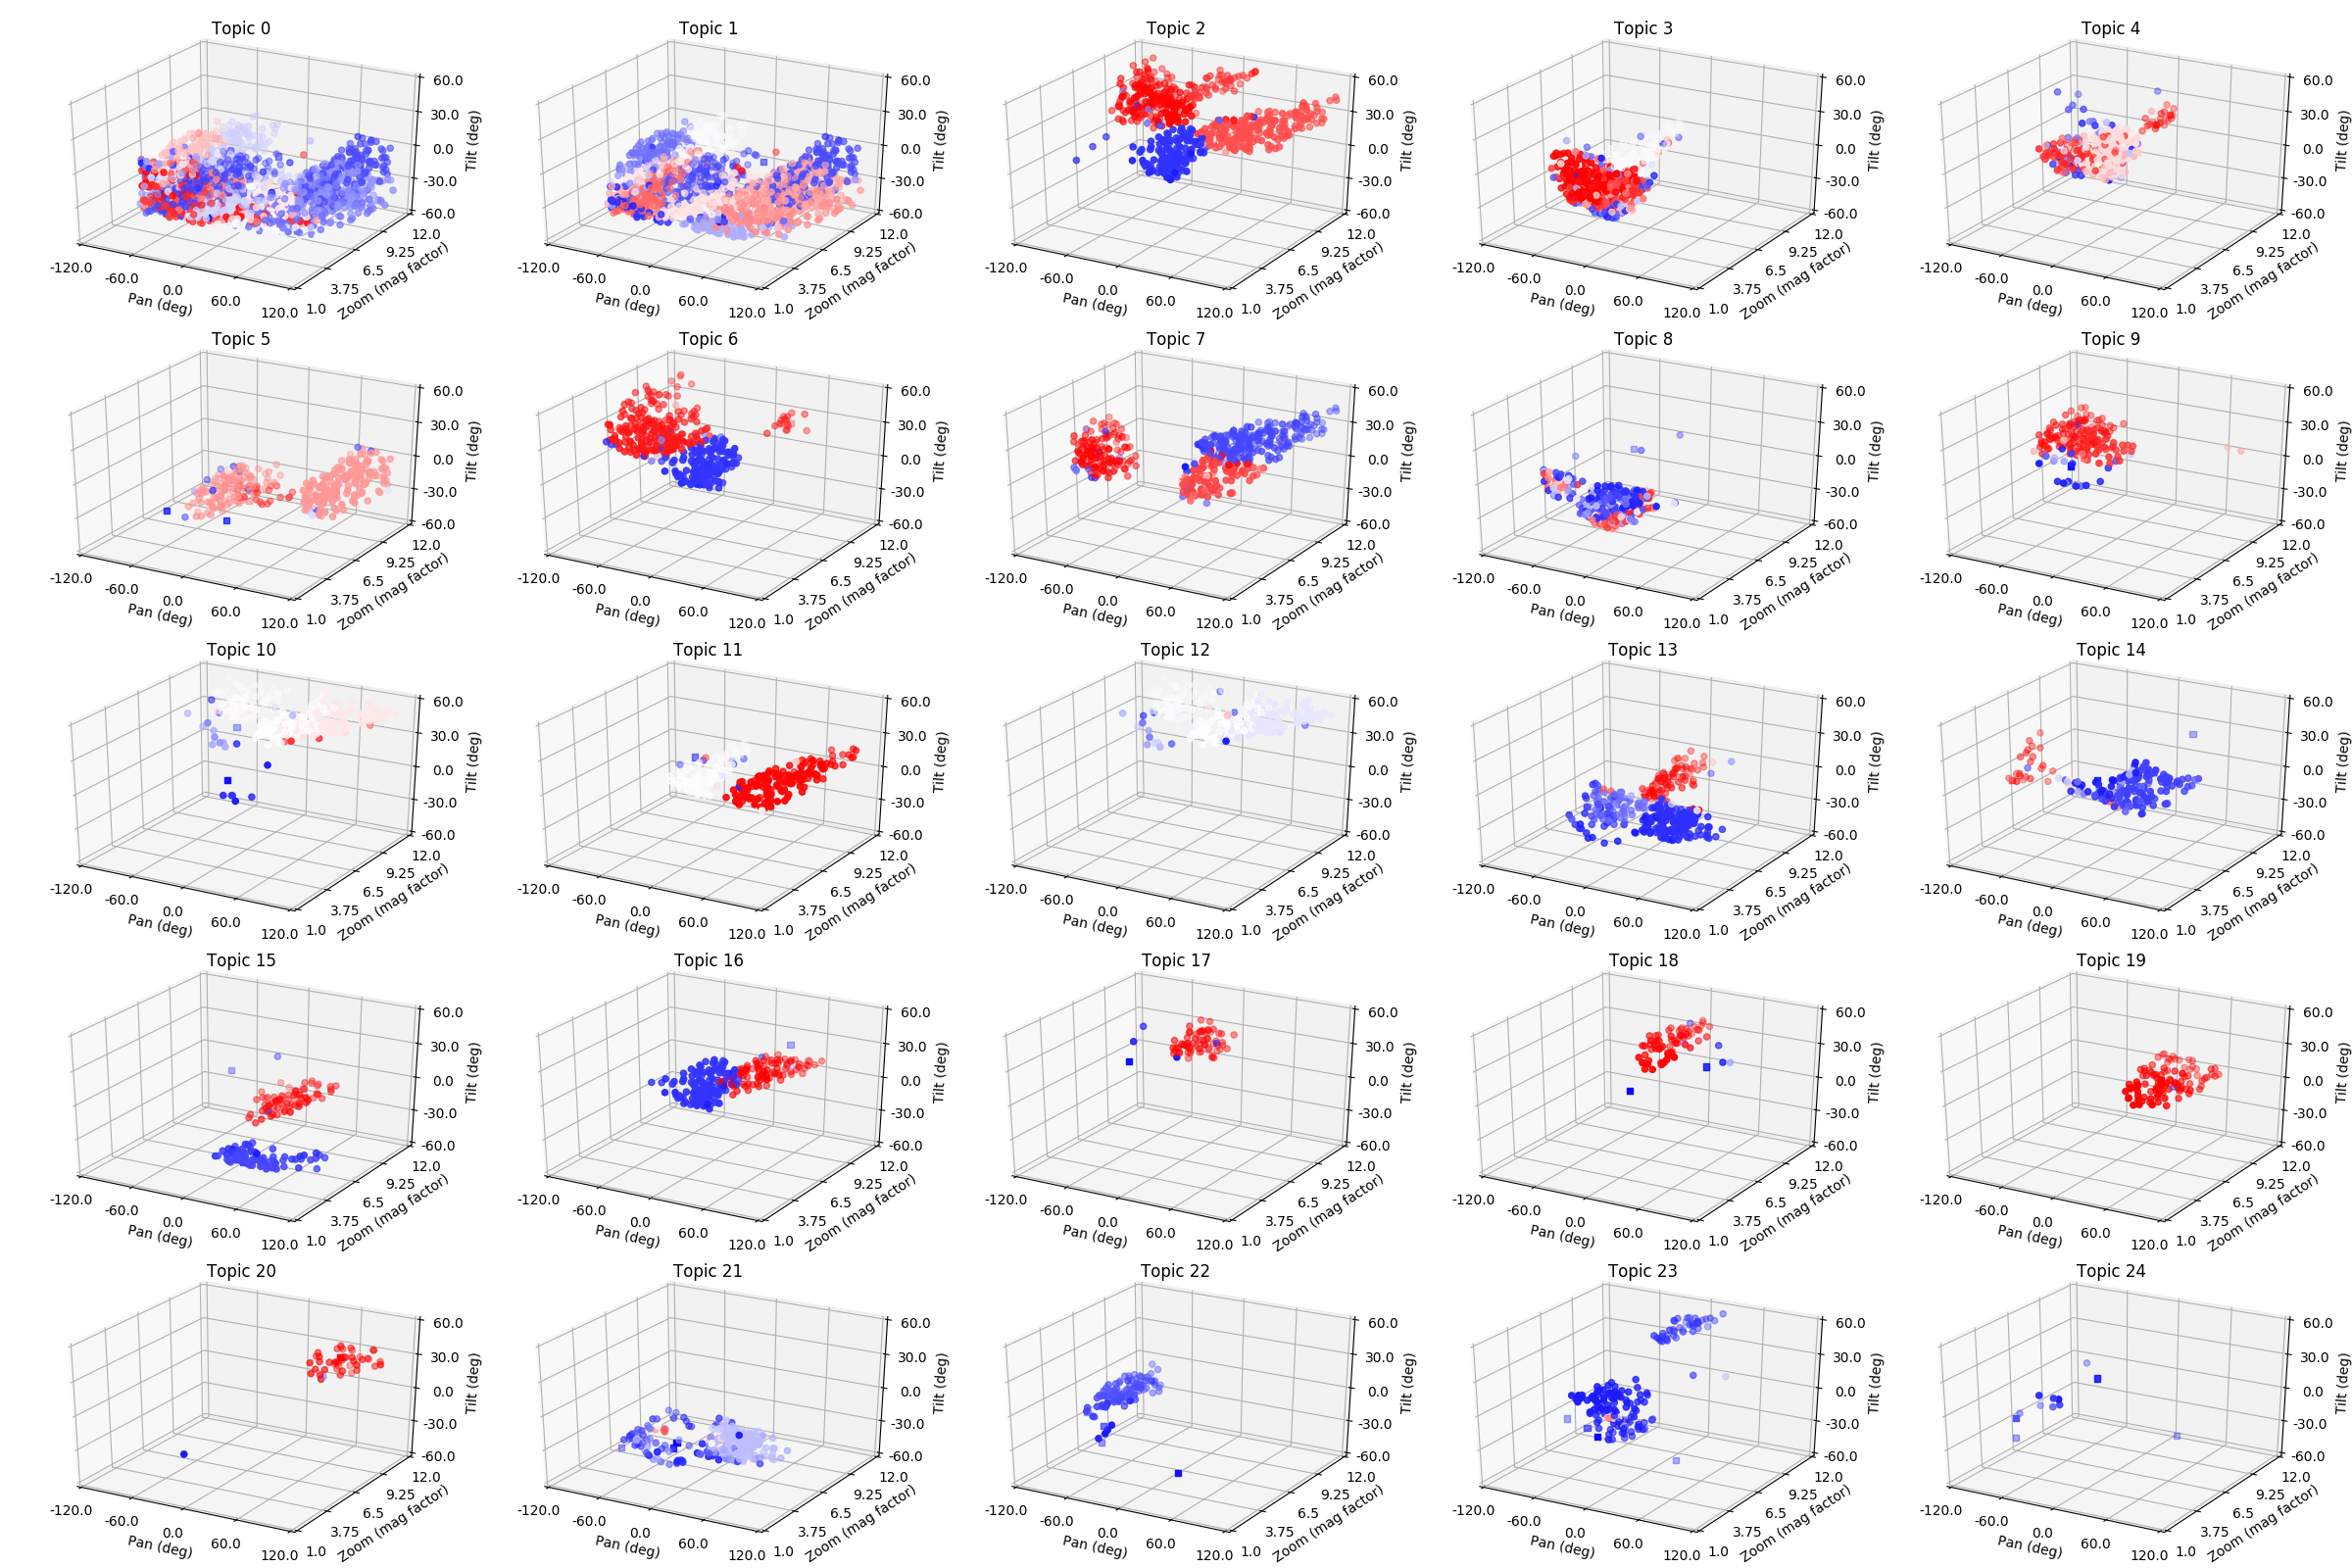
\includegraphics[width=\columnwidth]{figures/ptz/pano_24_map.png}
            \label{fig:pano-24-map}
        } \\
        \subfloat[][]{
            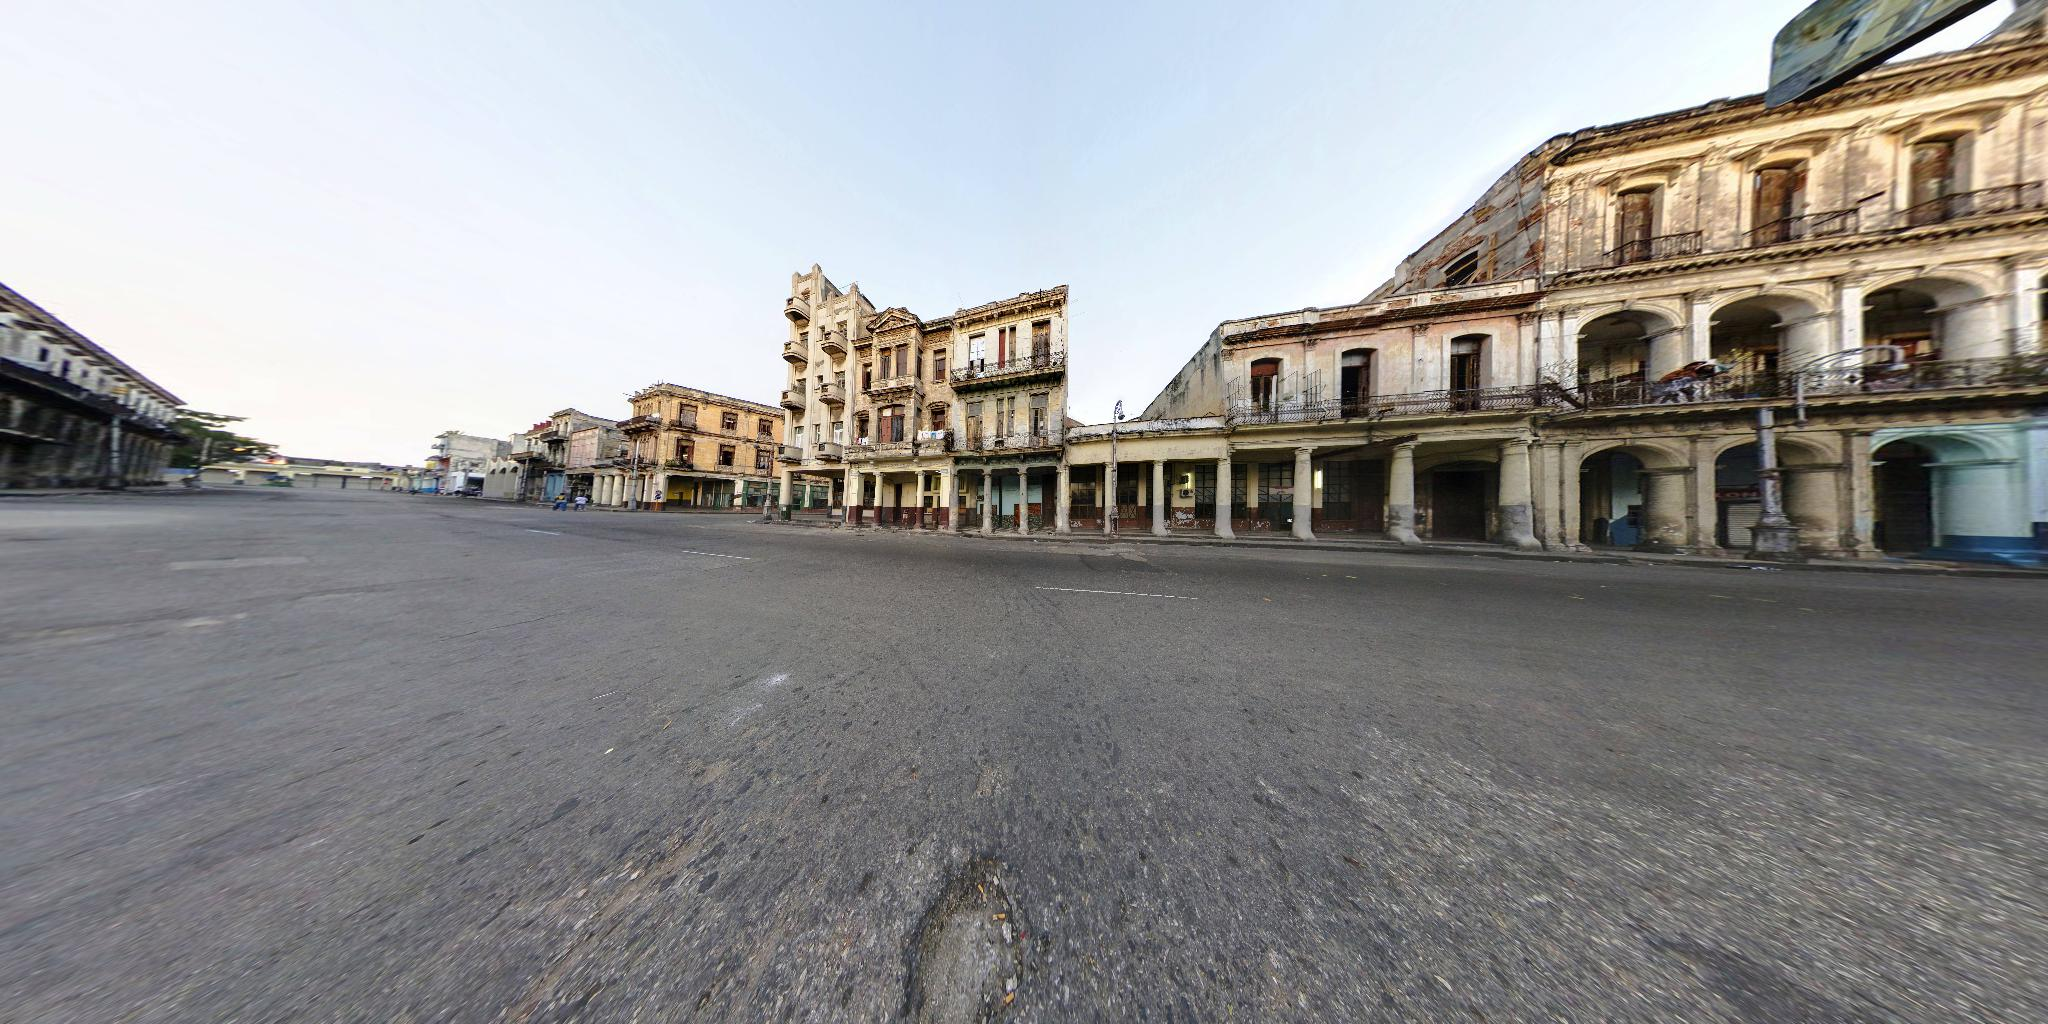
\includegraphics[width=\columnwidth]{figures/ptz/pano_24_pano.jpg}
            \label{fig:pano-24-pano}
        }
    \end{minipage}
    
    \caption{Example spatial prediction model after 50 training observations. \protect\subref{fig:pano-24-pano}} Fish-eye view of the entire panorama \protect\subref{fig:pano-24-topics}, Direct decoding of each topic-distribution ($\Phi_k$), And \protect\subref{fig:pano-24-map} predicted mixture of each topic.
    \label{fig:pano-24}
\end{figure}


\begin{figure}
    \begin{center}
    \subfloat[]{
        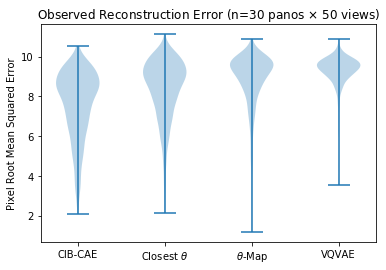
\includegraphics[width=0.48\columnwidth]{figures/ptz/vs_vqvae_obs.png}
        \label{fig:vs_vqvae_obs}
    }%
    \subfloat[]{
        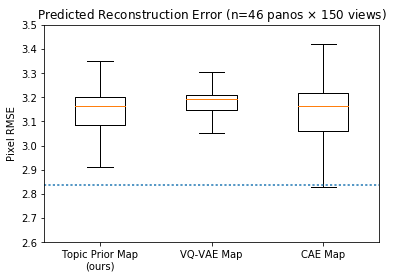
\includegraphics[width=0.48\columnwidth]{figures/ptz/vs_vqvae_pred.png}
        \label{fig:vs_vqvae_pred}
    }
    \end{center}
    \caption{ Comparison of topics autoencoder with vqvae.
    \protect\subref{fig:vs_vqvae_obs} Reconstructions of observed images
    \protect\subref{fig:vs_vqvae_pred} Predicted images after training with 50 uniform random pan-tilt-zoom poses.
    (MSEs are computed with respect to pixel values in the range [0,255])
    }
    \label{fig:vs_vqvae}
\end{figure}

\subsection{Visual topic-mixture search}

\section{Discussion}
Active learning \citep{Jayaraman2017}


